\chapter{Pràctica}
\label{cap:practica}

\section{El conjunt dels nombres reals}

\begin{exercici}
(1) Calcula la diagonal del rectangle les dimensions del qual són $2$ cm i $1$
cm, i (2) determina si el nombre que has obtingut és racional o
irracional.

\end{exercici}

\begin{solucio}
(1) Si designem per $x$ el valor de la diagonal, com que és rectangle el
triangle $ABC$
\begin{center}
  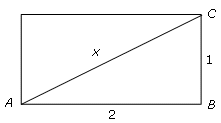
\includegraphics[width=2.3298in,height=1.3093in,keepaspectratio]{img/num24.png}
\end{center}
 podem aplicar el teorema de Pitàgores. D’aquesta manera, tenim%
\begin{equation*}
x^{2}=2^{2}+1^{2}=5
\end{equation*}%
Per tant, $x=\sqrt{5}$, és a dir, la diagonal del rectangle és un
segment de longitud $\sqrt{5}$ cm.

(2) Demostrarem per reducció a l’absurd que el nombre $\sqrt{5}$
es irracional. En altres paraules, suposant el contrari, és a dir, que $%
\sqrt{5}$ és racional, deduirem una contradicció. En efecte, si $%
\sqrt{5}$ és un nombre racional, aleshores podrem expressar-lo com una
fracció%
\begin{equation}
\sqrt{5}=\frac{n}{m}  \label{eq:sqrt5-fraccio}
\end{equation}%
on $n,m\in \mathbb{Z}$. No és restrictiu suposar que a més la fracció és irreductible, ja que, si no ho fos, la reduiríem a
una fracció irreductible equivalent. Per tant, els nombres enters 
$n$ i $m$ són primers entre si. A més, $m$ no pot ser $1$ ja que,
si ho fos, $\sqrt{5}$ seria un nombre enter i això no és possible
ja que, en la figura 1 hem situat $\sqrt{5}$ sobre la recta mitjançant
regla, escaire i compàs i hem comprovat que $\sqrt{5}$ és major que $%
2$ i menor que $3$.
\begin{center}
  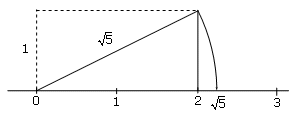
\includegraphics[width=3.1004in,height=1.2254in,keepaspectratio]{img/num23.png}
\par\smallskip
  \textbf{Figura 1}
\end{center}
Ara bé, es compleix (\ref{eq:sqrt5-fraccio}) si%
\begin{equation*}
\left( \frac{n}{m}\right) ^{2}=\frac{n^{2}}{m^{2}}=5
\end{equation*}%
però això no és possible ja que els nombres enters $n^{2}$ i $m^{2}$,
perquè són quadrats, tenen descomposicions en factors primers en què tots
els factors estan elevats al quadrat i, a més, en haver suposat
que $n$ i $m$ són primers entre si, no tenen cap factor en comú. Per tant, la fracció $\frac{n^{2}}{m^{2}}$ també és
irreductible i no es pot simplificar i ser igual a$5$.
\end{solucio}

\begin{exercici}
Un rectangle s’anomena auri quan té la propietat que si li
traiem un quadrat, el rectangle que queda és semblant al primer.%

\begin{center}
  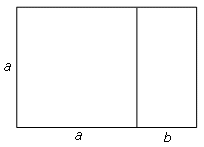
\includegraphics[width=2.1525in,height=1.5592in,keepaspectratio]{img/num21.png}
\end{center}
El quocient entre el costat major i el costat menor d’un rectangle auri s’anomena el nombre auri i es designa per $\Phi $.
(1) Calcula el nombre auri. (2) Prova que $\Phi$ és un nombre
irracional.

\end{exercici}

\begin{solucio}
(1) Com que són els rectangles $ABDE$ i $CDEF$ semblants, els seus costats seran proporcionals. Per tant, podem escriure%
\begin{equation*}
\Phi =\frac{\overline{AE}}{\overline{CF}}=\frac{\overline{AB}}{\overline{CD}}
\end{equation*}%

\begin{center}
  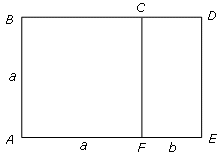
\includegraphics[width=2.3298in,height=1.663in,keepaspectratio]{img/num22.png}
\end{center}
és a dir,%
\begin{equation*}
\Phi =\frac{a+b}{a}=\frac{a}{b}
\end{equation*}%
De la proporció%
\begin{equation*}
\frac{a+b}{a}=\frac{a}{b}
\end{equation*}%
obtenim%
\begin{equation*}
1+\frac{b}{a}=\frac{a}{b}
\end{equation*}%
o, el que és el mateix,%
\begin{equation*}
1+\frac{1}{\frac{a}{b}}=\frac{a}{b}
\end{equation*}%
Ara bé, sabem que $\Phi =\frac{a}{b}$ i, per tant, podem escriure%
\begin{equation*}
1+\frac{1}{\Phi }=\Phi
\end{equation*}%
és a dir,%
\begin{equation*}
\frac{1}{\Phi }=\frac{\Phi -1}{1}
\end{equation*}%
d’on%
\begin{align*}
\Phi (\Phi -1) &=1 \\
\Phi ^{2}-\Phi &=1 \\
\Phi ^{2}-\Phi -1 &=0
\end{align*}%
Resolent aquesta equació de segon grau, obtenim les dues solucions
següents%
\begin{equation*}
\frac{1\pm \sqrt{1+4}}{2}=\frac{1\pm \sqrt{5}}{2}
\end{equation*}%
Tenint present que $\Phi$ designa un quocient entre longituds de
segments, $\Phi$ ha de ser un nombre positiu. Per tant, el nombre auri ve donat per%
\begin{equation*}
\Phi =\frac{1+\sqrt{5}}{2}
\end{equation*}

(2) Demostrarem per reducció a l’absurd que $\Phi$ és un nombre
irracional. Primer, observem que 
\begin{equation*}
\Phi =\frac{1+\sqrt{5}}{2}=\frac{1}{2}+\frac{1}{2}\cdot \sqrt{5}
\end{equation*}%
d’on s’obté%
\begin{equation}
\frac{\Phi -\frac{1}{2}}{\frac{1}{2}}=\sqrt{5}  \label{eq:phi-sqrt5}
\end{equation}%
Si fos $\Phi$ racional, com que és $\frac{1}{2}$ un nombre racional,
aleshores, per (\ref{eq:phi-sqrt5}), $\sqrt{5}$ seria un nombre racional,
però això no és possible, segons hem vist en l’exercici 1. D’aquesta
manera, deduïm que $\Phi$ és un nombre irracional.
\end{solucio}

\begin{exercici}
(1) Amb regla, escaire i compàs, representa sobre la rectals
següents nombres: a) $3(1-\sqrt{2})$, b) $2(3-\sqrt{2})$, c) $\frac{1}{%
2}(1+\sqrt{5})$. (2) Prova que els tres nombres anteriors són
irracionals.

\end{exercici}

\begin{solucio}
(1) Per resoldre aquesta qüestió, primer tracem una recta horitzontal.
Després situem l’origen i, a partir d’ell, situem la unitat.

a) Primer, construirem sobre la recta un segment de longitud $\sqrt{2}$.
Per això, amb l’ajuda de l’escaire dibuixem un triangle rectangle isòsceles de catets iguals a $1$. Pel teorema de Pitàgores, la seva hipotenusa serà $\sqrt{2}$. Amb l’ajuda del compàs,
situem $\sqrt{2}$ sobre la recta. Hem construït així un segment de
longitud $\sqrt{2}$, indicat en vermell en la figura 2
\begin{center}
  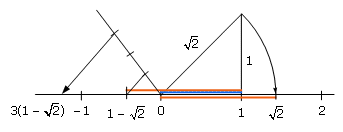
\includegraphics[width=3.6011in,height=1.4027in,keepaspectratio]{img/num26.png}
\par\smallskip
  \textbf{Figura 2}
\end{center}
Ara
situarem $1-\sqrt{2}$ sobre la recta. Per això, amb l’ajuda de la regla,
tracem un segment de longitud $\sqrt{2}$ a partir de $1$ cap a l’esquerra; per veure com s’ha fet, mira la figura 2. Finalment, fem
tres parts iguals sobre una recta qualsevol que passa per l’origen i,
unim amb una recta el punt $1-\sqrt{2}$ amb l’extrem de la primera
part. Ara, amb l’ajuda de la regla i l’escaire, tracem una recta
paral·lela des de l’extrem de la tercera part, pel teorema de Thales%
\footnote{%
Recorda que el teorema de Thales diu que els segments determinats sobre
dues rectes concurrents tallades per diverses rectes paral·leles són
proporcionals.}, el punt determinat per aquesta paral·lela sobre la recta serà $3(1-\sqrt{2})$; per veure com es fa això mira de nou la figura 2.

b) Procedirem de la mateixa manera per situar sobre la recta el nombre $2(3-%
\sqrt{2})$. Com a resum, adjuntem la figura 3, on es poden veure els
passos que s’han fet per situar $2(3-\sqrt{2})$.
\begin{center}
  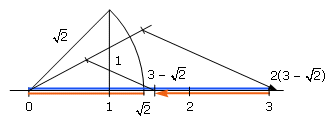
\includegraphics[width=3.4861in,height=1.3508in,keepaspectratio]{img/num27.png}
\par\smallskip
  \textbf{Figura 3}
\end{center}


c) De nou, cal aplicar el mètode explicat a l’apartat a). Com
resum, adjuntem la figura 4, on es poden veure els passos que s’han
fet per situar $\frac{1}{2}(1+\sqrt{5})$.
\begin{center}
  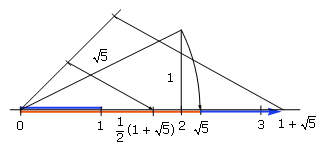
\includegraphics[width=3.3823in,height=1.6111in,keepaspectratio]{img/num28.png}
\par\smallskip
  \textbf{Figura 4}
\end{center}


(2) Per provar que els tres nombres anteriors són irracionals
utilitzarem el mètode de demostració per reducció a l’absurd.
Segons aquest mètode, es suposa el contrari i per raonaments
correctes hem de deduir una contradicció. En aquest cas, es conclou
que la hipòtesi que havíem negado és vertadera.

a) Sabem que $\sqrt{2}$ és un nombre irracional. Suposem que $3(1-%
\sqrt{2})$ és un nombre racional $r$, aleshores%
\begin{align*}
r &=3(1-\sqrt{2}) \\
\frac{r}{3} &=1-\sqrt{2} \\
\sqrt{2} &=1-\frac{r}{3}
\end{align*}%
però $1-\frac{r}{3}$ és un nombre racional, cosa que és absurda amb el
fet que $\sqrt{2}$ és un nombre irracional.

b) Procedirem de la mateixa manera, n’hi ha prou amb suposar que%
\begin{align*}
r &=2(3-\sqrt{2}) \\
\frac{r}{2} &=3-\sqrt{2} \\
\sqrt{2} &=3-\frac{r}{2}
\end{align*}%
i, com $3-\frac{r}{2}$ és un nombre racional, s’arriba a una contradicció, ja que, $\sqrt{2}$ és un nombre irracional.

c) Ens adonem que $\frac{1}{2}(1+\sqrt{5})$ és el nombre auri. En l’exercici 2, hem vist que aquest nombre és irracional.
\end{solucio}

\begin{exercici}
Utilitzant una calculadora que no té la tecla per calcular arrels, 
com trobaries una expressió decimal del nombre $\sqrt[3]{2}$ amb quatre xifres exactes?.

\end{exercici}

\begin{solucio}
Sabem que $x=\sqrt[3]{2}$ si $x^{3}=2$. D’aquesta manera, hem de trobar nombres tals que el seu cub sigui $2$. Per tempteig, mitjançant una calculadora,
obtenim els següents resultats per $\sqrt[3]{2}$:

\begin{center}
\begin{tabular}{l|l|l|l|l}
& {\small Grau d’aprox.} & $\sqrt[3]{2}${\small \ és major que} & $\sqrt[3]%
{2}${\small \ és menor que} & {\small Observacions} \\ \hline
{\small (1)} & {\small Unitats} & ${\small 1}$ & ${\small 2}$ & ${\small 1}%
^{3}{\small =1}${\small \ i }${\small 2}^{3}{\small =8}$ \\ 
{\small (2)} & {\small Dècimes} & ${\small 1.2}$ & ${\small 1.3}$ & $%
{\small 1.2}^{3}{\small =1.728}${\small \ i }${\small 1.3}^{3}{\small =2.197}
$ \\ 
{\small (3)} & {\small Centèsimes} & ${\small 1.25}$ & ${\small 1.26}$ & 
${\small 1.25}^{3}{\small =1.953125}${\small \ i }${\small 1.26}^{3}{\small%
=2.000376}$ \\ 
{\small (4)} & {\small Mil·lèsimes} & ${\small 1.259}$ & ${\small 1.260}$
& ${\small 1.259}^{3}{\small =1.995616979}${\small \ i }${\small 1.260}^{3}{\small =2.000376}$ \\ 
{\small (5)} & {\small Deumil·lèsimes} & ${\small 1.2599}$ & ${\small%
1.2600}$ & ${\small 1.2599}^{3}{\small =1.999899758}${\small \ i }${\small%
1.26}^{3}{\small =2.000376}$ \\ 
{\small (6)} & {\small Centmil·lèsimes} & ${\small 1.25992}$ & ${\small 1.25993}$ & ${\small 1.25992}^{3}{\small =1.999995000}${\small \ i }${\small 1.25993}^{3}{\small =2.000042622}$%
\end{tabular}
\end{center}

De (6) obtenim que $1.259$ és el valor aproximat de $\sqrt[3]{2}$ amb 4
xifres exactes.
\end{solucio}

\begin{exercici}
Classifica els següents nombres en naturals, enters, racionals,
irracionals, reals i no reals.%
\begin{equation*}
\sqrt{81},\sqrt[3]{81},-\frac{1}{2}\sqrt{63.999...},0.363636...,7.3,
\end{equation*}%
\begin{equation*}
\frac{13}{7},\sqrt{-25},-\sqrt{25},0.363663666...,\sqrt[3]{-25}
\end{equation*}

\end{exercici}

\begin{solucio}
Resumim els resultats mitjançant la taula següent:%
\begin{center}
\begin{tabular}{l|l|l|l|l|l|l}
{\small Nombre} & ${\small N}$ & ${\small Z}$ & ${\small Q}$ & ${\small I%
}$ & ${\small R}$ & {\small Observacions} \\ \hline
$\sqrt{{\small 81}}$ & {\small Sí} & {\small Sí} & {\small Sí}
& {\small No} & {\small Sí} & $\sqrt{{\small 81}}{\small =9}$ \\ 
$\sqrt[3]{{\small 81}}$ & {\small No} & {\small No} & {\small No} & {\small Sí} & {\small Sí} & {\small Nombre decimal no periòdic} \\ 
${\small -}\frac{1}{2}\sqrt{{\small 63.999...}}$ & {\small No} & {\small Sí} & {\small Sí} & {\small No} & {\small Sí} & ${\small -}%
\frac{1}{2}\sqrt{{\small 63.999...}}{\small =-}\frac{1}{2}\sqrt{{\small 64}}%
{\small =-}\frac{1}{2}{\small \cdot 8=-4}$ \\ 
${\small 0.363636...}$ & {\small No} & {\small No} & {\small Sí} & 
{\small No} & {\small Sí} & {\small Nombre decimal periòdic}
\\ 
${\small 7.3}$ & {\small No} & {\small No} & {\small Sí} & {\small No}
& {\small Sí} & {\small Nombre decimal exacte} \\ 
$\frac{13}{7}$ & {\small No} & {\small No} & {\small Sí} & {\small No}
& {\small Sí} & {\small Nombre decimal periòdic} \\ 
$\sqrt{{\small -25}}$ & {\small No} & {\small No} & {\small No} & {\small No}
& {\small No} & {\small No hi ha cap nombre real el quadrat del qual
sigui negatiu} \\ 
${\small -}\sqrt{{\small 25}}$ & {\small No} & {\small Sí} & {\small Sí} & {\small No} & {\small Sí} & ${\small -}\sqrt{{\small 25}}%
{\small =-5}$ \\ 
${\small 0.363663666...}$ & {\small No} & {\small No} & {\small No} & 
{\small Sí} & {\small Sí} & {\small Nombre decimal no periòdic} \\ 
$\sqrt[3]{{\small -25}}$ & {\small No} & {\small No} & {\small No} & {\small Sí} & {\small Sí} & {\small Nombre decimal negatiu no periòdic}%
\end{tabular}
\end{center}
\end{solucio}

\begin{exercici}
Considera la successió d’intervals encaixats definida per 
\begin{equation*}
\left[ \left( 1+\frac{1}{1}\right) ^{1},\left( 1+\frac{1}{1}\right) ^{2}%
\right] ,\left[ \left( 1+\frac{1}{2}\right) ^{2},\left( 1+\frac{1}{2}\right)
^{3}\right] ,...
\end{equation*}%
és a dir, els intervals són de la forma%
\begin{equation*}
\left[ \left( 1+\frac{1}{n}\right) ^{n},\left( 1+\frac{1}{n}\right) ^{n+1}%
\right]
\end{equation*}%
on $n=1,2,3,...$. Comprova que aquesta successió defineix el nombre
irracional anomenat \textbf{nombre }$e$, prenent $n=1$, $10$, $50$, $%
100$, $500$, $1000$, $10000$, $100000$ i $1000000$. Escriu les xifres
exactes del valor aproximat del nombre $e$ que pots obtenir a partir
dels valors indicats per $n$.

\end{exercici}

\begin{solucio}
Mitjançant una calculadora científica pots calcular de forma aproximada
el nombre $e$.%
\begin{equation*}
e=2.718281828
\end{equation*}%
Ara calculemos els intervals encaixats per $n=1$, $10$, $50$, $100$, $%
500 $, $1000$, $10000$, $100000$ i $1000000$.

\begin{equation*}
\begin{array}{c|c}
n & \left[ \left( 1+\frac{1}{n}\right) ^{n},\left( 1+\frac{1}{n}\right)
^{n+1}\right] \\ \hline
1 & \left[ 2,4\right] \\ 
10 & \left[ 2.59374246,2.853116706\right] \\ 
50 & \left[ 2.691588029,2.74541979\right] \\ 
100 & \left[ 2.704813829,2.731861968\right] \\ 
500 & \left[ 2.715568521,2.720999658\right] \\ 
1000 & \left[ 2.716923932,2.719640856\right] \\ 
10000 & \left[ 2.718145927,2.718417741\right] \\ 
100000 & \left[ 2.718268237,2.71829542\right] \\ 
1000000 & \left[ 2.718280469,2.718283188\right]%
\end{array}%
\end{equation*}

Per tant, 
\begin{equation*}
e=2.71828...
\end{equation*}
\end{solucio}

\begin{exercici}
Escriu les aproximacions decimals per defecte i per excés fins a l’ordre 
$5$ de $\sqrt{3}$ i de $1+\sqrt[3]{2}$. Amb quantes
xifres exactes pots escriure els valors aproximats d’aquests nombres?

\end{exercici}

\begin{solucio}
Amb una calculadora obtenim%
\begin{equation*}
\sqrt{3}=1.732050808\text{ \ \ i \ \ }1+\sqrt[3]{2}=2.25992105
\end{equation*}%
Aleshores les aproximacions decimals de $\sqrt{3}$ fins a l’ordre indicat,
són%
\begin{equation*}
\begin{array}{c|c|c}
\text{Ordre} & \text{Aprox. per defecte} & \text{Aprox. per excés} \\ \hline
1 & 1 & 2 \\ 
2 & 1.7 & 1.8 \\ 
3 & 1.73 & 1.74 \\ 
4 & 1.732 & 1.733 \\ 
5 & 1.7320 & 1.7321%
\end{array}%
\end{equation*}
i a partir d’aquests resultats, podem escriure el seu valor aproximat amb 4
xifres exactes%
\begin{equation*}
\sqrt{3}=1.732...
\end{equation*}%
Per $1+\sqrt[3]{2}$ tenim%
\begin{equation*}
\begin{array}{c|c|c}
\text{Ordre} & \text{Aprox. per defecte} & \text{Aprox. per excés} \\ \hline
1 & 2 & 3 \\ 
2 & 2.2 & 2.3 \\ 
3 & 2.25 & 2.26 \\ 
4 & 2.259 & 2.260 \\ 
5 & 2.2599 & 2.2600%
\end{array}%
\end{equation*}
i a partir d’aquí, podem escriure el seu valor aproximat amb 2 xifres
exactes%
\begin{equation*}
1+\sqrt[3]{2}=2.2...
\end{equation*}
\end{solucio}

\begin{exercici}
Situa sobre la recta real el nombre $\pi $.

\end{exercici}

\begin{solucio}
Per representar el nombre irracional $\pi$ de forma aproximada sobre
la recta real ho farem mitjançant aproximacions decimals, ja que no és
possible fer-ho amb regla i compàs. Amb l’ajuda d’una calculadora,
podem obtenir el següent valor aproximat 
\begin{equation*}
\pi =3.141592654
\end{equation*}%
Aleshores, prenent aproximacions decimals per defecte i per excés de $\pi $%
, tenim%
\begin{equation*}
\begin{array}{c|c|c}
\text{Ordre} & \text{Aprox. per defecte} & \text{Aprox. per excés} \\ \hline
1 & 3 & 4 \\ 
2 & 3.1 & 3.2 \\ 
3 & 3.14 & 3.15 \\ 
4 & 3.141 & 3.142 \\ 
\cdots & \cdots & \cdots%
\end{array}%
\end{equation*}%
Ara podem situar $\pi$ sobre la recta real de la següent manera:%

\begin{center}
  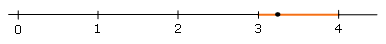
\includegraphics[width=4.0473in,height=0.486in,keepaspectratio]{img/num29.png}
\end{center}
augmentant l’interval $\left[ 3,4\right]$ de manera que puguem
visualitzar l’ordre aproximació de les dècimes, tenim
\begin{center}
  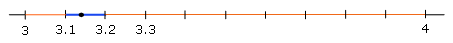
\includegraphics[width=4.7469in,height=0.4756in,keepaspectratio]{img/num30.png}
\end{center}
augmentant
l’interval $\left[ 3.1,3.2\right]$ de manera que puguem veure l’ordre d’
aproximació de les centèsimes, tenim
\begin{center}
  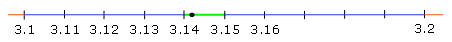
\includegraphics[width=4.7357in,height=0.4653in,keepaspectratio]{img/num31.png}
\end{center}
augmentant ara l’interval $\left[
3.14,3.15\right]$ de manera que puguem veure l’ordre d’aproximació de
les mil·lèsimes, tenim
\begin{center}
  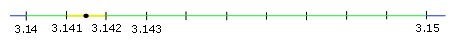
\includegraphics[width=4.7573in,height=0.4756in,keepaspectratio]{img/num32.png}
\end{center}
i així successivament, aquest
procés pot continuar fins a aconseguir situar-lo amb l’aproximació del
grau que ens interessi.
\end{solucio}

\begin{exercici}
Escriu tres nombres racionals i altres tres irracionals, compresos
entre 4 i 5, utilitzant fraccions i arrels. Justifica que els nombres que escriguis compleixen la condició imposada.

\end{exercici}

\begin{solucio}
Com a nombres racionals escollim, per exemple,%
\begin{equation*}
\frac{4+5}{2}=\frac{9}{2}=4.5
\end{equation*}%
que és el punt mitjà del segment $[4,5]$,%
\begin{equation*}
\frac{4+\frac{9}{2}}{2}=\frac{\frac{8+9}{2}}{2}=\frac{17}{4}=4.25
\end{equation*}%
que és el punt mitjà del segment $[4,\frac{9}{2}]$, i%
\begin{equation*}
\frac{\frac{9}{2}+5}{2}=\frac{\frac{19}{2}}{2}=\frac{19}{4}=4.75
\end{equation*}%
que és el punt mitjà del segment $[\frac{9}{2},5]$.

Com que $4^{2}=16$ i $5^{2}=25$, com nombres irracionals escollim,
per exemple,%
\begin{equation*}
\sqrt{17}=4.123105626
\end{equation*}%
\begin{equation*}
\sqrt{18}=4.242640687
\end{equation*}%
i%
\begin{equation*}
\sqrt{19}=4.358898944
\end{equation*}
\end{solucio}

\section{Les operacions en el conjunt dels nombres reals}

\begin{exercici}
De dos nombres reals $a$ i $b$ es coneix que $a=7.325...$ i $b=24.46...$%
. Dedueix entre què valors es trobaran $a+b$ i $a\cdot b$, i amb quantes xifres exactes podran donar-se en els resultats.

\end{exercici}

\begin{solucio}
Per simplificar l’escriptura utilitzarem la notació $a\leq b\leq c$
per indicar que el nombre real $b$ està comprès entre els nombres $a$ i $c$. Així, segons les dades, les aproximacions per
defecte i per excés de $a$ i $b$ són%
\begin{equation*}
7.325\leq a\leq 7.326\text{ \ \ i \ \ }24.46\leq b\leq 24.47
\end{equation*}%
Després,%
\begin{equation*}
7.325+24.46=31.785\leq a+b\leq 31.796=7.326+24.47
\end{equation*}%
i%
\begin{equation*}
7.325\cdot 24.46=179.1695\leq a\cdot b\leq 179.26722=7.326\cdot 24.47
\end{equation*}%
A la vista d’aquestes desigualtats, és clar que les úniques xifres
exactes per la suma són%
\begin{equation*}
a+b=31.7\cdots
\end{equation*}%
i pel producte,%
\begin{equation*}
a\cdot b=179.\cdots
\end{equation*}%
Observa que només podem assegurar l’exactitud de les xifres de la suma $%
a+b$ fins a les dècimes, és a dir, fins a l’ordre anterior al que
correspon l’última xifra exacta del sumand de menor precisió ($%
24.46...$, que és exacte fins a les centèsimes). Mentre que, en el
producte $a\cdot b$ només podem garantir tres xifres significatives,
és a dir, una xifra menys que el nombre de xifres significatives del factor
que menys té (tots dos tenen quatre xifres significatives).
\end{solucio}

\begin{exercici}
Utilitzant que $\sqrt{17}=4.1231046...$ i $\pi =3.1415926...$, calcula amb
aproximació fins a les mil·lèsimes, els nombres reals següents:
(1) $\sqrt{17}+\pi $, (2) $\sqrt{17}-\pi $, (3) $\sqrt{17}\cdot \pi $, i (4) 
$\sqrt{17}/\pi $.

\end{exercici}

\begin{solucio}
(1) Per obtenir $\sqrt{17}+\pi$ amb aproximació fins a les mil·lèsimes, s’han de prendre $\sqrt{17}$ i $\pi$ amb aproximació fins a les
deu mil·lèsimes. Aleshores,%
\begin{equation*}
\sqrt{17}+\pi =4.1231...+3.1415...=7.264\overset{?}{6}...=7.264...
\end{equation*}

(2) De la mateixa manera, per obtenir $\sqrt{17}-\pi$ amb aproximació fins a
les mil·lèsimes, s’han de prendre $\sqrt{17}$ i $\pi$ amb aproximació
fins a les deu mil·lèsimes. Aleshores,%
\begin{equation*}
\sqrt{17}-\pi =4.1231...-3.1415...=0.981\overset{?}{6}...=0.981...
\end{equation*}

(3) En trobar-se $\sqrt{17}\cdot \pi$ entre $12$ i $20$, ja que $4\leq 
\sqrt{17}\leq 5$ i $3\leq \pi \leq 4$, per obtenir aquest producte amb
aproximació fins a les mil·lèsimes, necessitem assegurar que cinc
(dues xifres enteres i tres xifres decimals) de les seves xifres siguin
significatives i, per tant, hem de prendre cada factor amb sis xifres
significatives. Aleshores,%
\begin{equation*}
\sqrt{17}\cdot \pi=\left( 4.12310...\right) \cdot \left(
3.14159...\right) =12.953\overset{?}{\overbrace{08973}...}=12.953...
\end{equation*}

(4) Com que $3\leq \pi \leq 4$, aleshores $\frac{1}{4}=0.25\leq \frac{1}{\pi }%
\leq 0.333...=\frac{1}{3}$; per tant, $\sqrt{17}/\pi$ es troba entre $%
1$ i $\frac{5}{3}=1.666...$. Per obtenir aquest quocient amb aproximació fins a les mil·lèsimes, necessitem assegurar que quatre (una xifra sencera
i tres xifres decimals) de les seves xifres siguin significatives i, per tant,
hem de prendre el numerador i el denominador amb cinc xifres significatives.
Aleshores,%
\begin{equation*}
\frac{\sqrt{17}}{\pi }=\frac{4.1231...}{3.1415...}=1.312\overset{?}{%
\overbrace{4622}}=1.312...
\end{equation*}
\end{solucio}

\begin{exercici}
Sabent que $a=-1.427...$ i $b=7.3902$, troba $a+b$, $a-b$, $a\cdot b$
i $\frac{a}{b}$, determinant la precisió de cada resultat.

\end{exercici}

\begin{solucio}
Segons les dades, les aproximacions per defecte i per excés de $a$ i $b$
són%
\begin{equation*}
-1.428\leq a\leq -1.427\text{ \ \ i \ \ }7.3902\leq b\leq 7.3903
\end{equation*}%
Després,%
\begin{equation*}
-1.428+7.3902=5.9622\leq a+b\leq 5.9633=-1.427+7.3903
\end{equation*}%
\begin{equation*}
-1.428-7.3903=-8.8183\leq a-b\leq -8.8172=-1.427-7.3902
\end{equation*}%
ja que $-7.3903\leq -b\leq -7.3902$, i, per tant, obtenim que%
\begin{equation*}
a+b=5.96...\text{ \ \ i \ \ }a-b=-8.81...
\end{equation*}%
és a dir, només podem assegurar l’exactitud de les xifres de la suma $%
a+b$ i la resta$a-b$ fins a les centèsimes, ja que el sumand de menor
precisió és exacte fins a les mil·lèsimes.

D’altra banda, tenim que%
\begin{equation*}
\left( -1.428\right) \cdot 7.3903=-10.5533484\leq a\cdot b\leq
-10.5458154=\left( -1.427\right) \cdot 7.3902
\end{equation*}%
i%
\begin{equation*}
\left( -1.428\right) \cdot 0.13532=-0.19323696\leq \frac{a}{b}\leq
-0.19308737=\left( -1.427\right) \cdot 0.13531
\end{equation*}%
ja que 
\begin{equation*}
\frac{1}{7.3903}=0.135312504\leq \frac{1}{b}\leq 0.135314335=\frac{1}{7.3902}
\end{equation*}%
és a dir,%
\begin{equation*}
\frac{1}{b}=0.13531...
\end{equation*}%
i, per tant, obtenim que%
\begin{equation*}
a\cdot b=-10.5...\text{ \ \ i \ \ }\frac{a}{b}=-0.193...
\end{equation*}%
és a dir, només podem garantir tres xifres significatives en el
producte, és a dir, una xifra menys que el nombre de xifres significatives
del factor $-1.427$ que menys té; en el quocient passa el mateix.
\end{solucio}

\begin{exercici}
Resol les següents qüestions: (1) calcula l’àrea d’un cercle de $3$ cm de radi i expressa el resultat amb tres decimals exactes;
(2) calcula l’àrea d’un triangle equilàter de $10$ cm de costat i
expressa el resultat amb dos decimals exactes.

\end{exercici}

\begin{solucio}
(1) Sabem que l’àrea d’un cercle de radi $r$ ve donada per
la fórmula%
\begin{equation*}
A=\pi r^{2}
\end{equation*}%
Com que $r=3$, tenim que%
\begin{equation*}
A=9\pi
\end{equation*}%
Com que $27\leq 9\pi \leq 36$, si volem expressar el resultat amb aproximació fins a les mil·lèsimes, necessitem assegurar que cinc (dues xifres
enteres i tres xifres decimals) de les seves xifres siguin significatives i, per
tant, hem de prendre $\pi$ amb sis xifres significatives. Com que $\pi
=3.14159...$, aleshores%
\begin{equation*}
A=9\cdot \left( 3.14159...\right) =28.274\overset{?}{\overbrace{31}}%
...=28.274...
\end{equation*}

(2) Si designem per $x$ l’altura d’aquest triangle, 
\begin{center}
  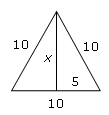
\includegraphics[width=1.1623in,height=1.2254in,keepaspectratio]{img/num43.png}
\end{center}
pel
teorema de Pitàgores, tenim%
\begin{equation*}
10^{2}=5^{2}+x^{2}
\end{equation*}%
és a dir,%
\begin{equation*}
x^{2}=75
\end{equation*}%
i, per tant, $x=\sqrt{75}$. Per tant, l’àrea del triangle
serà%
\begin{equation*}
A=\frac{1}{2}\cdot 10\cdot \sqrt{75}=5\sqrt{75}
\end{equation*}%
Com que $40\leq 5\sqrt{75}\leq 45$, si volem expressar el resultat amb
aproximació fins a les centèsimes, necessitem garantir que quatre
(dues xifres enteres i dos de decimals) de les seves xifres siguin significatives i,
per tant, hem de prendre $\sqrt{75}$ amb cinc xifres significatives. Com que $\sqrt{75}=8.6602...$, aleshores%
\begin{equation*}
A=5\cdot \left( 8.6602...\right) =43.30\overset{?}{1}=43.30...
\end{equation*}
\end{solucio}

\begin{exercici}
Considerem els nombres reals $\sqrt{13}$ i $\sqrt{17}$. Es demana: (1)
la seva representació sobre la recta real i (2) utilitzant procediments
geomètrics, representa també els següents nombres reals:
(a) $\sqrt{13}-\sqrt{17}$, (b) $\sqrt{13}\cdot \sqrt{17}/3$, i (c) $\sqrt{17}%
/\sqrt{13}$.

\end{exercici}

\begin{solucio}
(1) Observa primer que es compleixen les següents relacions%
\begin{equation*}
13=3^{2}+2^{2}\text{ \ \ i \ \ }17=4^{2}+1^{2}
\end{equation*}%
Ara, pel teorema de Pitàgores, podem construir segments de
longitud $\sqrt{13}$ i $\sqrt{17}$, utilitzant regla, escaire i compàs.
La següent figura mostra la construcció dels dos segments.
\begin{center}
  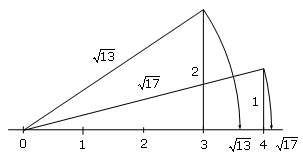
\includegraphics[width=3.1842in,height=1.6527in,keepaspectratio]{img/num39.png}
\end{center}


(2) Per resoldre les qüestions d’aquest apartat utilitzarem la
construccions geomètriques corresponents a les operacions amb
segments.

(a) Per representar $\sqrt{13}-\sqrt{17}$ sobre la recta real, fem la
construcció que s’indica a la figura següent.
\begin{center}
  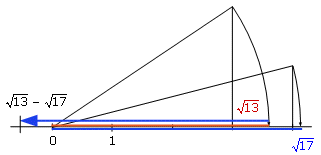
\includegraphics[width=3.3719in,height=1.6423in,keepaspectratio]{img/num40.png}
\end{center}


(b) Per obtenir 
\begin{equation*}
\frac{\sqrt{13}\cdot \sqrt{17}}{3}=\frac{\sqrt{13}}{3}\cdot \sqrt{17}
\end{equation*}%
fem la construcció que es mostra en la figura següent.
\begin{center}
  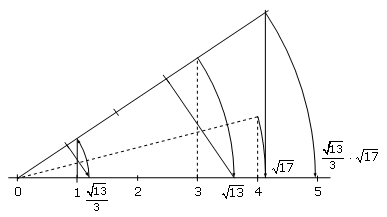
\includegraphics[width=4.0594in,height=2.2883in,keepaspectratio]{img/num41.png}
\end{center}


(c) Per representar 
\begin{equation*}
\frac{\sqrt{17}}{\sqrt{13}}=\sqrt{17}\cdot \frac{1}{\sqrt{13}}
\end{equation*}%
fem la construcció que s’indica a la figura següent.
\begin{center}
  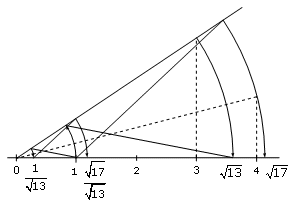
\includegraphics[width=3.1004in,height=2.1724in,keepaspectratio]{img/num42.png}
\end{center}

\end{solucio}

\begin{exercici}
Raona amb exemples les qüestions següents: (1) la suma de dos nombres irracionals, és sempre un nombre irracional?;
(2) el producte de dos nombres irracionals, és
sempre un nombre irracional? i (3) com és la
suma d’un nombre racional amb un irracional? i el
producte?

\end{exercici}

\begin{solucio}
(1) La suma de dos nombres irracionals no és sempre un nombre
irracional, ja que $\sqrt{2}$ i $-\sqrt{2}$ són dos nombres irracionals i
la seva suma $\sqrt{2}+(-\sqrt{2})=0$ no és un nombre irracional.

(2) El producte de dos nombres irracionals no és sempre un nombre
irracional, ja que $\sqrt{2}$ és un nombre irracional i el producte $\sqrt{%
2}\cdot \sqrt{2}=\left( \sqrt{2}\right) ^{2}=2$ és un nombre
racional.

(3) La suma d’un nombre racional $r$ amb un irracional $s$ és sempre
un irracional, ja que, altrament, $r+s$ seria un nombre
racional $r^{\prime }$ i, com a conseqüència, $s=r^{\prime }-r$ seria
també racional, cosa que no és possible per hipòtesi. De manera
similar, el producte d’un nombre racional no nul $r$ per un irracional 
$s$ és sempre un irracional, ja que, altrament, $r\cdot s$ seria
un nombre racional $r^{\prime }$ i, com a conseqüència, $s=\frac{%
r^{\prime }}{r}$ seria també racional, cosa que tampoc és possible
per hipòtesi.
\end{solucio}

\begin{exercici}
Observa el raonament següent i indica on és l’error:
suposem que $a\neq 0$ i que $a=b$. Aleshores, multiplicant ambdós costats de
la igualtat per $b$, obtenim $ab=b^{2}$. Sumant a ambdós membres de la
igualtat $-a^{2}$, obtenim $ab-a^{2}=b^{2}-a^{2}$. Ara, traient factor
comú $a$, a l’esquerra, i substituint $b^{2}-a^{2}$ per $(b+a)(b-a)$%
, a la dreta, obtenim%
\begin{equation*}
a(b-a)=(b+a)(b-a)
\end{equation*}%
Dividint ambdós membres de la igualtat per $b-a$, tenim%
\begin{equation*}
a=b+a
\end{equation*}%
però $a=b$, per tant $a=2a$. Finalment, en dividir ambdós costats de la igualtat
per $a$, deduïm que $1=2$.

\end{exercici}

\begin{solucio}
En passar de 
\begin{equation*}
a(b-a)=(b+a)(b-a)
\end{equation*}
a 
\begin{equation*}
a=b+a
\end{equation*}
es comet l’error de dividir per $b-a=0$, ja que, $a=b$, cosa que no és possible.
\end{solucio}

\begin{exercici}
Resol les equacions següents, indicant les propietats que utilitzes
en cada pas de la resolució: (1) $3(5-2x)+4x-3=6-(4-2x)$; (2) $%
(x-1)(x^{2}-5)=0$; i (3) $x^{2}+16=0$.

\end{exercici}

\begin{solucio}
(1) 
\begin{align*}
3(5-2x)+4x-3 &=6-(4-2x) \\
15-6x+4x-3 &=6-4+2x \\
12-2x &=2+2x \\
-2x-2x &=-12+2 \\
-4x &=-10 \\
4x &=10 \\
2x &=5 \\
x &=\frac{5}{2}
\end{align*}

(2)%
\begin{equation*}
(x-1)(x^{2}-5)=0
\end{equation*}%
Per tractar-se d’un producte de dos factors que és igual a zero, els nombres reals que satisfan l’equació anterior han de complir que%
\begin{equation*}
x+1=0\text{ \ \ o \ \ }x^{2}-5=0
\end{equation*}%
De l’equació $x+1=0$, es dedueix $x=-1$, i de l’altra equació, $%
x^{2}-5=0$, equivalent a $x^{2}=5$, es dedueixen dos valors per $x$, $\sqrt{%
5}$ i $-\sqrt{5}$; això és així perquè%
\begin{equation*}
\left( \sqrt{5}\right) ^{2}=5\text{ \ \ i \ \ }\left( -\sqrt{5}\right)
^{2}=\left( \sqrt{5}\right) ^{2}=5
\end{equation*}%
Per tant, les solucions de l’equació són $-1$, $\sqrt{5}$ i $-%
\sqrt{5}$.

(3) L’equació $x^{2}+16=0$ és equivalent a $x^{2}=-16$, però no hi ha
cap nombre real que el quadrat del qual sigui negatiu. Per tant,
l’equació no té solució en $\mathbb{R}$.
\end{solucio}

\begin{exercici}
Si $x,y$ són nombres reals qualssevol, provar que es compleix la
següent identitat%
\begin{equation*}
x^{3}\pm y^{3}=(x\pm y)(x^{2}\mp xy+y^{2})
\end{equation*}

\end{exercici}

\begin{solucio}
Provarem que es compleix 
\begin{equation*}
x^{3}-y^{3}=(x-y)(x^{2}+xy+y^{2})
\end{equation*}%
i deixem com a exercici l’altra identitat. Tenim que%
\begin{align*}
(x-y)(x^{2}+xy+y^{2}) &=x(x^{2}+xy+y^{2})-y(x^{2}+xy+y^{2}) \\
&=x^{3}+x^{2}y+xy^{2}-yx^{2}-xy^{2}-y^{3} \\
&=x^{3}-y^{3}
\end{align*}
\end{solucio}

\begin{exercici}
Prova que l’equació de segon grau $ax^{2}+bx+c=0$ té com
solucions 
\begin{equation*}
x=\frac{-b\pm \sqrt{b^{2}-4ac}}{2a}
\end{equation*}

\end{exercici}

\begin{solucio}
En efecte, puaixò que $a\neq 0$ i suposant que $b^{2}-4ac\geq 0$, tenim%
\begin{align*}
ax^{2}+bx+c &=0 \\
4a\cdot (ax^{2}+bx+c) &=4a\cdot 0 \\
4a^{2}x^{2}+4abx+4ac &=0 \\
4a^{2}x^{2}+4abx+4ac+b^{2} &=b^{2} \\
4a^{2}x^{2}+4abx+4ac+b^{2}-4ac &=b^{2}-4ac \\
4a^{2}x^{2}+4abx+b^{2} &=b^{2}-4ac \\
(2ax+b)^{2} &=b^{2}-4ac \\
2ax+b &=\pm \sqrt{b^{2}-4ac} \\
2ax+b-b &=\pm \sqrt{b^{2}-4ac}-b \\
2ax &=-b\pm \sqrt{b^{2}-4ac} \\
x &=\frac{-b\pm \sqrt{b^{2}-4ac}}{2a}
\end{align*}
\end{solucio}

\section{L’ordre en el conjunt dels nombres reals}

\begin{exercici}
Si $a,b$ són dos nombres reals positius, provar que es compleix%
\begin{equation*}
\begin{array}{ccc}
a^{2}<b^{2} & \Longrightarrow & a<b%
\end{array}%
\end{equation*}%
Si $a,b$ no són positius, és certa la implicación
anterior?

\end{exercici}

\begin{solucio}
Evidentment, es compleix%
\begin{align*}
a^{2} &<&b^{2} \\
0 &<&b^{2}-a^{2} \\
0 &<&(a+b)(a-b)
\end{align*}%
Com que per hipòtesi $a,b\in \mathbb{R}^{+}$, es compleix $a+b\in 
\mathbb{R}^{+}$ i, per tant, de l’última desigualtat, es dedueix $%
a-b\in \mathbb{R}^{+}$, és a dir, $a<b$.

Si $a,b$ no són positius, la implicación no és certa, ja que, per
exemple,%
\begin{equation*}
(-2)^{2}=4<9=(-3)^{2}
\end{equation*}%
i no és cert que $-2$ sigui menor que $-3$.
\end{solucio}

\begin{exercici}
Si $a,b$ són dos nombres reals positius, provar que es compleix%
\begin{equation*}
\sqrt{a\cdot b}\leq \frac{a+b}{2}
\end{equation*}%
En què casos es dona la igualtat?

\end{exercici}

\begin{solucio}
Observa que si $a>0$, $b>0$ i $a\neq b$, aleshores $\sqrt{a}>0$, $\sqrt{b}>0$
i $\sqrt{a}\neq \sqrt{b}$. Aleshores, es compleix%
\begin{align*}
\left( \sqrt{a}-\sqrt{b}\right) ^{2} &>&0 \\
\left( \sqrt{a}\right) ^{2}-2\sqrt{a}\cdot \sqrt{b}+\left( \sqrt{b}\right)
^{2} &>&0 \\
a-2\sqrt{a\cdot b}+b &>&0 \\
a+b &>&2\sqrt{a\cdot b} \\
\frac{a+b}{2} &>&\sqrt{a\cdot b}
\end{align*}%
Per tant, la desigualtat estricta es compleix quan $a\neq b$. Si $a=b>0$%
, aleshores la desigualtat es converteix en una igualtat, ja que, els dos
membres són iguals a$a$.

Per altra banda, suposem $a>0$, $b>0$ i que es compleix%
\begin{align*}
\sqrt{a\cdot b} &=\frac{a+b}{2} \\
ab &=\frac{(a+b)^{2}}{4} \\
4ab &=(a+b)^{2} \\
4ab &=a^{2}+2ab+b^{2} \\
0 &=a^{2}-2ab+b^{2} \\
0 &=(a-b)^{2}
\end{align*}%
d’on es dedueix que $a=b$. Per tant, la igualtat es compleix quan $a=b$.
\end{solucio}

\begin{exercici}
Sigui $A=\{x\in \mathbb{R}:x<4\}$, $B=\{x\in \mathbb{R}:x\geq -4\}$ i $%
C=\{x\in \mathbb{R}:0<x<7\}$. (a) Expressa els conjunts donats en forma de
intervals o semirectes; (b) expressa$A\cap B\cap C$ en forma d’entorn de
algun punt.

\end{exercici}

\begin{solucio}
(a) És clar que%
\begin{equation*}
\begin{array}{l}
A=(-\infty ,4) \\ 
B=[-4,+\infty ) \\ 
C=(0,7)%
\end{array}%
\end{equation*}

(b) Primer calcularem $A\cap B\cap C$. Per això, observa la figura
següent:
\begin{center}
  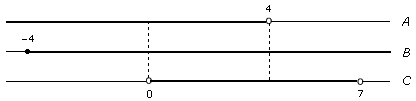
\includegraphics[width=4.3613in,height=1.0802in,keepaspectratio]{img/num52.png}
\end{center}
És clar a partir d’ella que%
\begin{equation*}
A\cap B\cap C=(0,4)
\end{equation*}%
El punt mitjà d’aquest interval és $2$ i la distància d’aquest a un
qualsevol dels extrems és també 2. Per tant,%
\begin{equation*}
A\cap B\cap C=E_{2}(2)
\end{equation*}
\end{solucio}

\begin{exercici}
Calcula el suprem, ínfim, màxim i mínim (si existeixen) dels
següents conjunts:

\begin{enumerate}
\item[a)] $A=(-\infty ,3)\cup \lbrack 10,11)$

\item[b)] $B=\{x\in \mathbb{R}:x^{2}-4x+3<0\}$

\item[c)] $C=\{x\in \mathbb{R}:\left\vert x-1\right\vert \leq 3\}$

\item[d)] $D=\{1/n:n\in \mathbb{N}\}$
\end{enumerate}

\end{exercici}

\begin{solucio}
a) És clar que el conjunt 
\begin{equation*}
A=(-\infty ,3)\cup \lbrack 10,11)
\end{equation*}
noestà fitat inferiorment i que els punts del conjunt $[11,+\infty
)$ són cotes superiors de $A$. Per això no existeix $\inf A$ i $\sup A=11$.
A més, $A$ no admet màxim ni mínim.

b) Primer, expressaremos 
\begin{equation*}
B=\{x\in \mathbb{R}:x^{2}-4x+3<0\}
\end{equation*}
mitjançant intervals o semirectes. Per això, hem de resoldre la següent
inequació de segon%
\begin{equation*}
x^{2}-4x+3<0
\end{equation*}%
Un mètode per resoldre aquest tipus d’inequacions és representar
de manera aproximada la paràbola $y=x^{2}-4x+3$ i esbrinar després per a quins valors de $x$ és $y<0$. Busquem els punts de tall de la paràbola amb l’eix $OX$, resolent l’equació%
\begin{equation*}
x^{2}-4x+3=0
\end{equation*}%
les solucions de les quals són $x=1$ o $x=3$. Per la simetria de la paràbola
i pel fet que $a=1>0$, en $x=2$ la paràbola tindrà un mínim com
es mostra a la figura següent. 
\begin{center}
  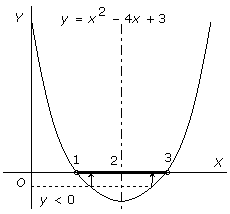
\includegraphics[width=2.4232in,height=2.2572in,keepaspectratio]{img/num53.png}
\end{center}
A partir de la gràfica, és clar
que $y<0$ quan $1<x<3$. Per tant,%
\begin{equation*}
B=(1,3)
\end{equation*}%
A partir d’aquí, és clar que $\sup B=3$, $\inf B=1$ i que $B$ no
admet màxim ni mínim.

c) Observa, en primer lloc, que%
\begin{align*}
\left\vert x-1\right\vert &\leq &3 \\
-3 &\leq &x-1\leq 3 \\
-2 &\leq &x\leq 4
\end{align*}%
Després,%
\begin{align*}
C &=\{x\in \mathbb{R}:\left\vert x-1\right\vert \leq 3\} \\
&=[-2,4]
\end{align*}%
D’aquí, es dedueix de forma immediata que $\sup C=\max C=4$ i $\inf
C=\min C=-2$.

d) Ara tenim que%
\begin{equation*}
D=\{1/n:n\in \mathbb{N}\}
\end{equation*}%
Observa que%
\begin{equation*}
\frac{1}{n}>0
\end{equation*}%
per a tot $n\in \mathbb{N}$. Per tant, $0$ és una cota inferior de $D$.
Observa també que%
\begin{equation*}
\frac{1}{n}\leq 1
\end{equation*}%
per a tot $n\in \mathbb{N}$. Per tant, $1$ és una cota superior de $D$. A
partir d’aquests dos fets, és evident que $\sup D=\max D=1$, $\inf D=0$ i $%
D$ no admet mínim.
\end{solucio}

\begin{exercici}
Escriu les expressions següents senes far uso del valor absolut:

\begin{enumerate}
\item[a)] $\left\vert x-3\right\vert $

\item[b)] $\left\vert x-1\right\vert +\left\vert x+3\right\vert $

\item[c)] $\left\vert 1-\left\vert x\right\vert \right\vert $

\item[d)] $\left\vert x-y\right\vert -\left\vert y\right\vert $
\end{enumerate}

\end{exercici}

\begin{solucio}
Per resoldre aquestes qüestions hem de recordar la definició de valor
absolut:%
\begin{equation*}
\left\vert a\right\vert =\left\{ 
\begin{array}{ll}
a & \text{si }a\geq 0 \\ 
-a & \text{si }a<0%
\end{array}%
\right.
\end{equation*}

a) L’expressió $\left\vert x-3\right\vert$ dependrà del signe de $%
x-3$; si $x\geq 3$, aleshores $x-3\geq 0$, i si $x<3$, aleshores $x-3<0$. Per
tant,%
\begin{equation*}
\left\vert x-3\right\vert =\left\{ 
\begin{array}{ll}
x-3 & \text{si }x\geq 3 \\ 
-(x-3)=3-x & \text{si }x<3%
\end{array}%
\right.
\end{equation*}

b) L’expressió $\left\vert x-1\right\vert +\left\vert x+3\right\vert $
dependrà dels signes de $x-1$ i $x+3$. Observa la següent figura:%

\begin{center}
  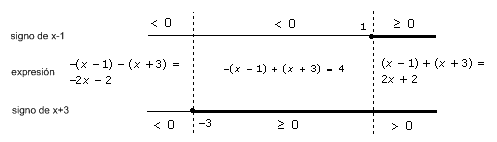
\includegraphics[width=5.2044in,height=1.5074in,keepaspectratio]{img/num54.png}
\end{center}
A partir d’ella, és clar que es compleix%
\begin{equation*}
\left\vert x-1\right\vert +\left\vert x+3\right\vert =\left\{ 
\begin{array}{ll}
2x+2 & \text{si }x\geq 1 \\ 
4 & \text{si }-3\leq x<1 \\ 
-2x-2 & \text{si }x<3%
\end{array}%
\right.
\end{equation*}

c) L’expressió $\left\vert 1-\left\vert x\right\vert \right\vert $
dependrà, primer, del signe de $x$. Així, tenim%
\begin{equation*}
\left\vert 1-\left\vert x\right\vert \right\vert =\left\{ 
\begin{array}{ll}
\left\vert 1-x\right\vert & \text{si }x\geq 0 \\ 
\left\vert 1-(-x)\right\vert =\left\vert 1+x\right\vert & \text{si }x<0%
\end{array}%
\right.
\end{equation*}%
Aleshores, si $x\geq 0$, tenim%
\begin{equation*}
\left\vert 1-x\right\vert =\left\{ 
\begin{array}{ll}
1-x & \text{si }0<x\leq 1 \\ 
-(1-x)=x-1 & \text{si }x>1%
\end{array}%
\right.
\end{equation*}%
i si $x<0$, tenim%
\begin{equation*}
\left\vert 1+x\right\vert =\left\{ 
\begin{array}{ll}
1+x & \text{si }-1\leq x<0 \\ 
-(1+x)=-1-x & \text{si }x<-1%
\end{array}%
\right.
\end{equation*}%
En resum, hem obtingut que%
\begin{equation*}
\left\vert 1-\left\vert x\right\vert \right\vert =\left\{ 
\begin{array}{ll}
x-1 & \text{si }x>1 \\ 
1-x & \text{si }0<x\leq 1 \\ 
1+x & \text{si }-1\leq x<0 \\ 
-1-x & \text{si }x<-1%
\end{array}%
\right.
\end{equation*}

d) L’expressió $\left\vert x-y\right\vert -\left\vert y\right\vert $
dependrà dels signes de $x-y$ i $y$. Observa les regions del pla
assenyalades a la figura següent:
\begin{center}
  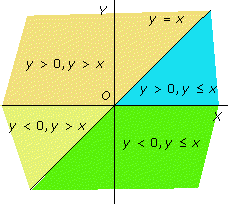
\includegraphics[width=2.4025in,height=2.1525in,keepaspectratio]{img/num55.png}
\end{center}
A partir d’elles, és clar que es compleix%
\begin{equation*}
\left\vert x-y\right\vert -\left\vert y\right\vert =\left\{ 
\begin{array}{ll}
-(x-y)-y=-x & \text{si }y>0,y>x \\ 
x-y-y=x-2y & \text{si }y>0,y\leq x \\ 
-(x-y)-(-y)=-x+2y & \text{si }y<0,y>x \\ 
x-y-(-y)=x & \text{si }y<0,y\leq x%
\end{array}%
\right.
\end{equation*}
\end{solucio}

\begin{exercici}
Resol les següents equacions:

\begin{enumerate}
\item[a)] $\left\vert x+1\right\vert =\left\vert 2x-3\right\vert $

\item[b)] $\left\vert x+1\right\vert +\left\vert x-1\right\vert =4$

\item[c)] $\left\vert x^{2}-x\right\vert +\left\vert x\right\vert =9$
\end{enumerate}

\end{exercici}

\begin{solucio}
Per resoldre aquestes equacions, primer examinaremos els signes de les
expressions amb valor absolut per saber quan l’expressió canvia
de signe o queda igual. Segon, resoldrem les equacions que resulten en
cada regió i, tercer, descartarem les solucions que no pertanyen a
les regiones corresponents.

a) Per resoldre l’equació $\left\vert x+1\right\vert =\left\vert
2x-3\right\vert$ cal examinar els signes de les expressions $x+1$ i $%
2x-3$. Per això, observa la següent figura:
\begin{center}
  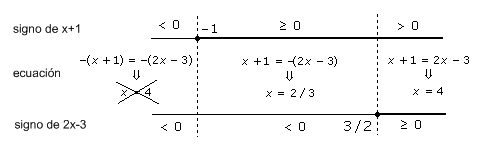
\includegraphics[width=5.0176in,height=1.5696in,keepaspectratio]{img/num56.png}
\end{center}
D’ella es desprèn que les
solucions són $x=2/3$ o $x=4$.

b) De la mateixa manera resoldrem l’equació $\left\vert x+1\right\vert
+\left\vert x-1\right\vert =4$. Observa la següent figura per veure els
signes de les expressions $x+1$ i $x-1$:
\begin{center}
  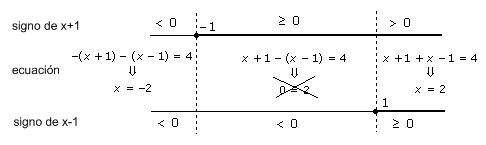
\includegraphics[width=5.0903in,height=1.5385in,keepaspectratio]{img/num57.png}
\end{center}
A partir d’ella, és clar que les
solucions són $x=-2$ o $x=2$.

c) Anàlogament, per resoldre l’equació $\left\vert
x^{2}-x\right\vert +\left\vert x\right\vert =9$ hem de analizar els signes
de les expressions $x^{2}-x$ i $x$. Per això, observa la següent figura:%

\begin{center}
  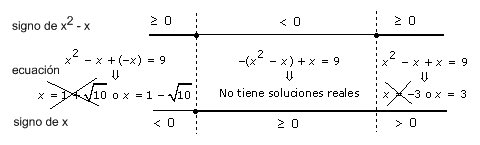
\includegraphics[width=5.028in,height=1.5385in,keepaspectratio]{img/num58.png}
\end{center}
A partir d’ella, és clar que les solucions són $x=1-\sqrt{10}$
o $x=3$.
\end{solucio}

\begin{exercici}
Resol les inequacions següents, expressent les solucions en forma de
intervals o semirectes:

\begin{enumerate}
\item[a)] $\left\vert 3-x\right\vert \geq \left\vert 2x+1\right\vert $

\item[b)] $\left\vert x-1\right\vert +\left\vert x+2\right\vert >3$

\item[c)] $2<\left\vert 4-x^{2}\right\vert \leq 12$

\item[d)] $\left\vert \frac{x-1}{x+1}\right\vert <2$

\item[e)] $\left\vert 4-\frac{1}{x^{2}}\right\vert <1$
\end{enumerate}

\end{exercici}

\begin{solucio}
Per resoldre aquestes inequacions utilitzarem la mateixa tècnica usada en
el exercici 24, és a dir, primer examinaremos els signes de les
expressions amb valor absolut per saber quan l’expressió canvia
de signe o queda igual. Segon, resoldrem les inequacions que resulten
en cada regió i, tercer, descartarem les solucions que no
pertanyen a les regiones corresponents.

a) Per resoldre la inequació $\left\vert 3-x\right\vert \geq
\left\vert 2x+1\right\vert $, observa la figura següent:
\begin{center}
  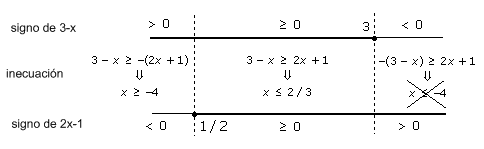
\includegraphics[width=5.0695in,height=1.58in,keepaspectratio]{img/num59.png}
\end{center}
A partir
de ella, és clar que les solucions són $-4\leq x\leq 2/3$, és a dir, els
punts de l’interval tancat%
\begin{equation*}
\left[ -4,2/3\right]
\end{equation*}

b) Per resoldre la inequació $\left\vert x-1\right\vert +\left\vert
x+2\right\vert >3$, observa la figura següent:
\begin{center}
  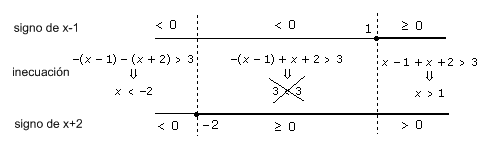
\includegraphics[width=5.0903in,height=1.5489in,keepaspectratio]{img/num60.png}
\end{center}
A partir d’ella, és clar que les
solucions són $x<-2$ o $x>1$, és a dir, els punts de la següent unió de semirectes obertes%
\begin{equation*}
\left( -\infty ,-2\right) \cup \left( 1,+\infty \right)
\end{equation*}

c) Per resoldre la inequació $2<\left\vert 4-x^{2}\right\vert \leq 12$%
, observa la figura següent:
\begin{center}
  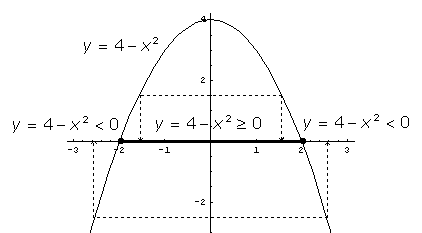
\includegraphics[width=4.4235in,height=2.4543in,keepaspectratio]{img/num62.png}
\end{center}
En ella hem representat la paràbola $y=4-x^{2}$ per poder esbrinar el signe de l’expressió $4-x^{2}$%
. Veiem que si $-2\leq x\leq 2$, aleshores $4-x^{2}\geq 0$, i en el cas contrari, $%
4-x^{2}<0$. Hi ha, doncs, dos casos: (1) $-2\leq x\leq 2$ i (2) $x<-2$ o $x>2$.

(1) Suposem que $-2\leq x\leq 2$, aleshores en aquesta regió la inequació s’escriu com%
\begin{equation*}
\begin{array}{c}
2<4-x^{2}\leq 12 \\ 
-2<-x^{2}\leq 8 \\ 
2>x^{2}\geq -8%
\end{array}%
\end{equation*}%
d’on resulta $x^{2}<2$, ja que, $x^{2}\geq -8$ es compleix per tot $x\in 
\mathbb{R}$. Per tant, les solucions són%
\begin{equation*}
-\sqrt{2}<x<\sqrt{2}
\end{equation*}%
com es pot deduir de la següent figura
\begin{center}
  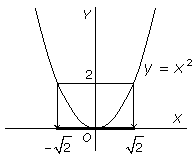
\includegraphics[width=2.0591in,height=1.6725in,keepaspectratio]{img/num63.png}
\end{center}
Observa que les solucions que hem
obtingudes són dins de la regió considerada.

(2) Suposem ara que $x<-2$ o $x>2$, aleshores en aquesta regió la
inequació s’escriu com%
\begin{equation*}
\begin{array}{c}
2<-(4-x^{2})\leq 12 \\ 
2<-4+x^{2}\leq 12 \\ 
6<x^{2}\leq 16%
\end{array}%
\end{equation*}%
d’on resulten les inequacions $x^{2}\leq 16$ i $x^{2}>6$. De la
primera, obtenim $-4\leq x\leq 4$, i de la segona, $x<-\sqrt{6}$ o $x>\sqrt{6}$%
. Igual que abans, aquests resultats es poden deduir de la representació gràfica de la paràbola $y=x^{2}$. De les solucions obtingudes
només les que indiquem a continuació%
\begin{equation*}
-4\leq x<-\sqrt{6}\text{ \ \ \ i \ \ \ }\sqrt{6}<x\leq 4
\end{equation*}%
estan en la regió considerada. En resum, les solucions de la
inequació $2<\left\vert 4-x^{2}\right\vert \leq 12$ són tots els nombres reals pertanyents a la següent unió d’intervals%
\begin{equation*}
\lbrack -4,-\sqrt{6})\cup (-\sqrt{2},\sqrt{2})\cup (\sqrt{6},4]
\end{equation*}%
En la figura següent s’assenyala un altre mètode per resoldre aquest tipus
d’inequacions, basat en la representació gràfica de la corba$%
y=\left\vert 4-x^{2}\right\vert$ a partir de la paràbola $y=4-x^{2}$. 

\begin{center}
  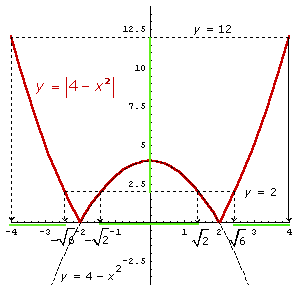
\includegraphics[width=3.1531in,height=3.1211in,keepaspectratio]{img/num61.png}
\end{center}
Observa com s’obtenen les mateixes solucions.

(d) Per resoldre la inequació 
\begin{equation*}
\left\vert \frac{x-1}{x+1}\right\vert <2
\end{equation*}%
primer efectuamos les següents transformacions%
\begin{align*}
\frac{\left\vert x-1\right\vert }{\left\vert x+1\right\vert } &<&2 \\
\left\vert x-1\right\vert &<&2\left\vert x+1\right\vert
\end{align*}%
en el supòsit de que $x\neq -1$. Observa ara la següent figura:
\begin{center}
  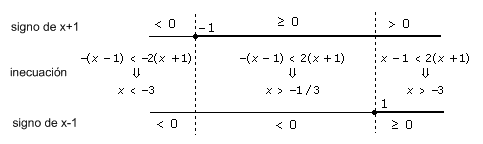
\includegraphics[width=5.0583in,height=1.5281in,keepaspectratio]{img/num64.png}
\end{center}
A partir
de ella, obtenim que les solucions de la inequació són $x<-3$ o $%
x>-1/3$, ja que, en la regió $x\geq 1$ la inequació es compleix
trivialment (perquè $x\geq 1>-3$), és a dir, els punts de la següent unión de semirectes%
\begin{equation*}
\left( -\infty ,-3\right) \cup \left( -1/3,+\infty \right)
\end{equation*}

e) Per resoldre la inequació%
\begin{equation*}
\left\vert 4-\frac{1}{x^{2}}\right\vert <1
\end{equation*}%
primer efectuamos les següents transformacions 
\begin{align*}
\left\vert \frac{4x^{2}-1}{x^{2}}\right\vert &<&1 \\
\frac{\left\vert 4x^{2}-1\right\vert }{\left\vert x^{2}\right\vert } &<&1 \\
\frac{\left\vert 4x^{2}-1\right\vert }{x^{2}} &<&1 \\
\left\vert 4x^{2}-1\right\vert &<&x^{2}
\end{align*}%
en el supòsit de que $x\neq 0$. En la següent figura hem dibuixat la paràbola $y=4x^{2}-1$ per poder esbrinar el signe de l’expressió $%
4x^{2}-1$. 
\begin{center}
  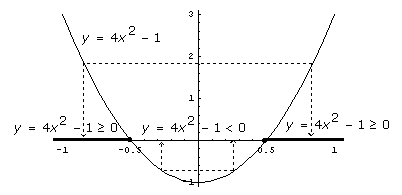
\includegraphics[width=4.2151in,height=2.0591in,keepaspectratio]{img/num65.png}
\end{center}
Observa que per $x\leq -1/2$ o $x\geq 1/2$ es compleix $%
4x^{2}-1\geq 0$, i en el cas contrari es compleix $4x^{2}-1<0$. Hi ha, doncs, dos casos:
(1) $x\leq -1/2$ o $x\geq 1/2$ i (2) $-1/2<x<1/2$.

(1) Suposem que $x\leq -1/2$ o $x\geq 1/2$, aleshores en aquesta regió
la inequació s’escriu així%
\begin{align*}
4x^{2}-1 &<&x^{2} \\
3x^{2} &<&1 \\
x^{2} &<&\frac{1}{3}
\end{align*}%
les solucions de les quals són%
\begin{equation*}
-1/\sqrt{3}<x<1/\sqrt{3}
\end{equation*}%
com es pot deduir en seguida a partir de la gràfica de la paràbola $y=x^{2}$. Per tant, les solucions que estan dins de la regió considerada són%
\begin{equation}
-1/\sqrt{3}<x\leq -1/2\text{ \ \ o \ \ }1/2\leq x<1/\sqrt{3}  \label{eq:ineq-franja-1}
\end{equation}

(2) Suposem ara que $-1/2<x<1/2$, aleshores en aquesta regió la
inequació s’escriu així%
\begin{align*}
-(4x^{2}-1) &<&x^{2} \\
-4x^{2}+1 &<&x^{2} \\
1 &<&5x^{2} \\
\frac{1}{5} &<&x^{2}
\end{align*}%
les solucions de les quals són%
\begin{equation*}
x<-1/\sqrt{5}	ext{ o }x>1/\sqrt{5}
\end{equation*}%
com es pot deduir en seguida a partir de la gràfica de la paràbola $y=x^{2}$. De les solucions obtingudes, només estan dins de la
regió considerada les que indiquem a continuació%
\begin{equation}
1/\sqrt{5}<x<1/2\text{ \ \ \ \ o \ \ \ }-1/2<x<-1/\sqrt{5}  \label{eq:ineq-franja-2}
\end{equation}%
En resum, ajuntant les solucions (\ref{eq:ineq-franja-1}) i (\ref{eq:ineq-franja-2}), obtenim que
les solucions de la inequació dada són tots els nombres reals de
la següent unió d’intervals oberts%
\begin{equation*}
\left( -1/\sqrt{3},-1/\sqrt{5}\right) \cup \left( 1/\sqrt{5},1/\sqrt{3}%
\right)
\end{equation*}
\end{solucio}

\section{Potències enteres de nombres reals}

\begin{exercici}
Calcular:

\begin{enumerate}
\item[a)] 
\begin{equation*}
\left[ \left( -\frac{1}{3}\right) ^{5}\cdot \left( \frac{1}{3}\right)
^{2}\cdot \left( -\frac{1}{3}\right) ^{3}\right] :\left[ \left( -\frac{1}{3}%
\right) ^{4}\cdot \left( \frac{1}{3}\right) ^{5}\right]
\end{equation*}

\item[b)] 
\begin{equation*}
\frac{\left( 0.25\right) ^{3}\cdot \left( -\frac{1}{4}\right) ^{2}}{\left( -%
\frac{1}{2}\right) ^{3}\cdot \left( 0.5\right) ^{2}}
\end{equation*}

\item[c)] 
\begin{equation*}
\frac{5^{3}\cdot \left( \frac{1}{25}\right) ^{2}\cdot 5^{7}}{5^{4}\cdot
\left( \frac{1}{5}\right) ^{2}}
\end{equation*}

\item[d)] 
\begin{equation*}
\frac{\left( \frac{1}{3}\right) ^{7}\cdot \left( -\frac{1}{4}\right)
^{2}\cdot \left( \frac{1}{9}\right) ^{4}}{\left[ \left( \frac{1}{9}\right)
^{2}\right] ^{3}\cdot \frac{1}{27}}
\end{equation*}
\end{enumerate}

\end{exercici}

\begin{solucio}
a)%
\begin{align*}
\left[ \left( -\frac{1}{3}\right) ^{5}\cdot \left( \frac{1}{3}\right)
^{2}\cdot \left( -\frac{1}{3}\right) ^{3}\right] &:&\left[ \left( -\frac{1}{3%
}\right) ^{4}\cdot \left( \frac{1}{3}\right) ^{5}\right] =\frac{\left[
-\left( \frac{1}{3}\right) ^{5}\right] \cdot \left( \frac{1}{3}\right)
^{2}\cdot \left[ -\left( \frac{1}{3}\right) ^{3}\right] }{\left( \frac{1}{3}%
\right) ^{4}\cdot \left( \frac{1}{3}\right) ^{5}} \\
&=\frac{\left( \frac{1}{3}\right) ^{10}}{\left( \frac{1}{3}\right) ^{9}} \\
&=\frac{1}{3}
\end{align*}

b)%
\begin{align*}
\frac{\left( 0.25\right) ^{3}\cdot \left( -\frac{1}{4}\right) ^{2}}{\left( -%
\frac{1}{2}\right) ^{3}\cdot \left( 0.5\right) ^{2}} &=\frac{\left( \frac{1%
}{4}\right) ^{3}\cdot \left( \frac{1}{4}\right) ^{2}}{\left[ -\left( \frac{1%
}{2}\right) ^{3}\right] \cdot \left( \frac{1}{2}\right) ^{2}} \\
&=\frac{\left( \frac{1}{4}\right) ^{5}}{-\left( \frac{1}{2}\right) ^{5}} \\
&=-\frac{\left[ \left( \frac{1}{2}\right) ^{2}\right] ^{5}}{\left( \frac{1}{%
2}\right) ^{5}} \\
&=-\frac{\left( \frac{1}{2}\right) ^{10}}{\left( \frac{1}{2}\right) ^{5}} \\
&=-\left( \frac{1}{2}\right) ^{5} \\
&=-\frac{1}{2^{5}} \\
&=-\frac{1}{32}
\end{align*}

c)%
\begin{align*}
\frac{5^{3}\cdot \left( \frac{1}{25}\right) ^{2}\cdot 5^{7}}{5^{4}\cdot
\left( \frac{1}{5}\right) ^{2}} &=\frac{5^{10}\cdot \left[ \left( \frac{1}{5%
}\right) ^{2}\right] ^{2}}{5^{4}\cdot \frac{1}{5^{2}}} \\
&=\frac{5^{10}\cdot \left( \frac{1}{5}\right) ^{4}}{\frac{5^{4}}{5^{2}}} \\
&=\frac{5^{10}\cdot \frac{1}{5^{4}}}{5^{2}} \\
&=\frac{\frac{5^{10}}{5^{4}}}{5^{2}} \\
&=\frac{5^{6}}{5^{2}} \\
&=5^{4} \\
&=625
\end{align*}

d)%
\begin{align*}
\frac{\left( \frac{1}{3}\right) ^{7}\cdot \left( -\frac{1}{4}\right)
^{2}\cdot \left( \frac{1}{9}\right) ^{4}}{\left[ \left( \frac{1}{9}\right)
^{2}\right] ^{3}\cdot \frac{1}{27}} &=\frac{\left( \frac{1}{3}\right)
^{7}\cdot \left( \frac{1}{4}\right) ^{2}\cdot \left[ \left( \frac{1}{3}%
\right) ^{2}\right] ^{4}}{\left( \frac{1}{9}\right) ^{6}\cdot \left( \frac{1%
}{3}\right) ^{3}} \\
&=\frac{\left( \frac{1}{3}\right) ^{7}\cdot \left( \frac{1}{4}\right)
^{2}\cdot \left( \frac{1}{3}\right) ^{8}}{\left[ \left( \frac{1}{3}\right)
^{2}\right] ^{6}\cdot \left( \frac{1}{3}\right) ^{3}} \\
&=\frac{\left( \frac{1}{3}\right) ^{15}\cdot \left( \frac{1}{4}\right) ^{2}%
}{\left( \frac{1}{3}\right) ^{12}\cdot \left( \frac{1}{3}\right) ^{3}} \\
&=\frac{\left( \frac{1}{3}\right) ^{15}\cdot \left( \frac{1}{4}\right) ^{2}%
}{\left( \frac{1}{3}\right) ^{15}} \\
&=\left( \frac{1}{4}\right) ^{2} \\
&=\frac{1}{16}
\end{align*}
\end{solucio}

\begin{exercici}
Calcular:

\begin{enumerate}
\item[a)] 
\begin{equation*}
\frac{\left( a^{2}\cdot b\cdot c\right) ^{3}\cdot \left( a\cdot b^{2}\cdot
c^{3}\right) ^{4}}{\left( \frac{a^{2}\cdot b}{b^{2}\cdot c}\right) ^{2}\cdot
\left( \frac{a\cdot b}{c}\right) ^{3}}
\end{equation*}

\item[b)] 
\begin{equation*}
\frac{\left[ \left( \frac{1}{a^{2}\cdot b}\right) ^{2}\right] ^{3}\cdot
\left( \frac{a^{3}\cdot b\cdot c}{b^{3}}\right) ^{2}}{\left( \frac{a\cdot
b\cdot c}{b^{3}}\right) ^{2}:\left( \frac{b\cdot c}{a^{2}}\right) ^{2}}
\end{equation*}
\end{enumerate}

\end{exercici}

\begin{solucio}
a)%
\begin{align*}
\frac{\left( a^{2}\cdot b\cdot c\right) ^{3}\cdot \left( a\cdot b^{2}\cdot
c^{3}\right) ^{4}}{\left( \frac{a^{2}\cdot b}{b^{2}\cdot c}\right) ^{2}\cdot
\left( \frac{a\cdot b}{c}\right) ^{3}} &=\frac{\left( a^{2}\right)
^{3}\cdot b^{3}\cdot c^{3}\cdot a^{4}\cdot (b^{2})^{4}\cdot (c^{3})^{4}}{%
\frac{(a^{2}\cdot b)^{2}}{(b^{2}\cdot c)^{2}}\cdot \frac{(a\cdot b)^{3}}{%
c^{3}}} \\
&=\frac{a^{6}\cdot b^{3}\cdot c^{3}\cdot a^{4}\cdot b^{8}\cdot c^{12}}{%
\frac{(a^{2})^{2}\cdot b^{2}}{b^{4}\cdot c^{2}}\cdot \frac{a^{3}\cdot b^{3}}{%
c^{3}}} \\
&=\frac{a^{10}\cdot b^{11}\cdot c^{15}}{\frac{a^{4}\cdot b^{2}\cdot
a^{3}\cdot b^{3}}{b^{4}\cdot c^{2}\cdot c^{3}}} \\
&=\frac{a^{10}\cdot b^{11}\cdot c^{15}}{\frac{a^{7}\cdot b^{5}}{b^{4}\cdot
c^{5}}} \\
&=\frac{a^{10}\cdot b^{11}\cdot c^{15}}{1}:\frac{a^{7}\cdot b}{c^{5}} \\
&=\frac{a^{10}\cdot b^{11}\cdot c^{15}\cdot c^{5}}{a^{7}\cdot b} \\
&=a^{3}\cdot b^{10}\cdot c^{20}
\end{align*}

b)%
\begin{align*}
\frac{\left[ \left( \frac{1}{a^{2}\cdot b}\right) ^{2}\right] ^{3}\cdot
\left( \frac{a^{3}\cdot b\cdot c}{b^{3}}\right) ^{2}}{\left( \frac{a\cdot
b\cdot c}{b^{3}}\right) ^{2}:\left( \frac{b\cdot c}{a^{2}}\right) ^{2}} &=%
\frac{\left( \frac{1}{a^{2}\cdot b}\right) ^{6}\cdot \frac{(a^{3}\cdot
b\cdot c)^{2}}{(b^{3})^{2}}}{\frac{(a\cdot b\cdot c)^{2}}{(b^{3})^{2}}:\frac{%
(b\cdot c)^{2}}{(a^{2})^{2}}} \\
&=\frac{\frac{1}{(a^{2}\cdot b)^{6}}\cdot \frac{a^{6}\cdot b^{2}\cdot c^{2}%
}{b^{6}}}{\frac{a^{2}\cdot b^{2}\cdot c^{2}}{b^{6}}:\frac{b^{2}\cdot c^{2}}{%
a^{4}}} \\
&=\frac{\frac{1}{a^{12}\cdot b^{6}}\cdot \frac{a^{6}\cdot b^{2}\cdot c^{2}}{%
b^{6}}}{\frac{a^{2}\cdot b^{2}\cdot c^{2}\cdot a^{4}}{b^{6}\cdot b^{2}\cdot
c^{2}}} \\
&=\frac{\frac{a^{6}\cdot b^{2}\cdot c^{2}}{a^{12}\cdot b^{6}\cdot b^{6}}}{%
\frac{a^{6}\cdot b^{2}\cdot c^{2}}{b^{8}\cdot c^{2}}} \\
&=\frac{a^{6}\cdot b^{2}\cdot c^{2}\cdot b^{8}\cdot c^{2}}{a^{12}\cdot
b^{12}\cdot a^{6}\cdot b^{2}\cdot c^{2}} \\
&=\frac{a^{6}\cdot b^{10}\cdot c^{4}}{a^{18}\cdot b^{14}\cdot c^{2}} \\
&=\frac{c^{2}}{a^{12}\cdot b^{4}}
\end{align*}
\end{solucio}

\begin{exercici}
Demostrar que si $a$ i $b$ són dos nombres qualssevol no nuls,
aleshores%
\begin{equation*}
\left( \frac{a}{b}\right) ^{-n}=\left( \frac{b}{a}\right) ^{n}
\end{equation*}

\end{exercici}

\begin{solucio}
En efecte,%
\begin{align*}
\left( \frac{a}{b}\right) ^{-n} &=\frac{1}{\left( \frac{a}{b}\right) ^{n}}
\\
&=\frac{1}{\frac{a^{n}}{b^{n}}} \\
&=\frac{b^{n}}{a^{n}} \\
&=\left( \frac{b}{a}\right) ^{n}
\end{align*}
\end{solucio}

\begin{exercici}
Calcular

\begin{enumerate}
\item[a)] 
\begin{equation*}
\frac{(0.1)^{-7}\cdot \left( \frac{1}{10}\right) ^{-5}}{\left( \frac{1}{100}%
\right) ^{2}\cdot \left[ \left( -0.001\right) ^{-3}\right] ^{2}}
\end{equation*}

\item[b)] 
\begin{equation*}
\frac{\left( \frac{1}{3}\right) ^{5}\cdot \left( -\frac{1}{3}\right)
^{-4}\cdot \left( \frac{1}{9}\right) ^{2}}{\left( \frac{1}{9}\right)
^{-2}\cdot \left( \frac{1}{27}\right) ^{-3}}
\end{equation*}
\end{enumerate}

\end{exercici}

\begin{solucio}
a)%
\begin{align*}
\frac{(0.1)^{-7}\cdot \left( \frac{1}{10}\right) ^{-5}}{\left( \frac{1}{100}%
\right) ^{2}\cdot \left[ \left( -0.001\right) ^{-3}\right] ^{2}} &=\frac{%
\left( \frac{1}{10}\right) ^{-7}\cdot \left( \frac{1}{10}\right) ^{-5}}{%
\left[ \left( \frac{1}{10}\right) ^{2}\right] ^{2}\cdot \left( -\frac{1}{1000%
}\right) ^{-6}} \\
&=\frac{\left( \frac{1}{10}\right) ^{-12}}{\left( \frac{1}{10}\right)
^{4}\cdot \left[ -\left( \frac{1}{10}\right) ^{3}\right] ^{-6}} \\
&=\frac{\left( \frac{1}{10}\right) ^{-12}}{\left( \frac{1}{10}\right)
^{4}\cdot (-1)^{-6}\cdot \left( \frac{1}{10}\right) ^{-18}} \\
&=\frac{\left( \frac{1}{10}\right) ^{-12}}{\left( \frac{1}{10}\right) ^{-14}%
} \\
&=\left( \frac{1}{10}\right) ^{2} \\
&=\frac{1}{100}
\end{align*}

b)%
\begin{align*}
\frac{\left( \frac{1}{3}\right) ^{5}\cdot \left( -\frac{1}{3}\right)
^{-4}\cdot \left( \frac{1}{9}\right) ^{2}}{\left( \frac{1}{9}\right)
^{-2}\cdot \left( \frac{1}{27}\right) ^{-3}} &=\frac{\left( \frac{1}{3}%
\right) ^{5}\cdot \left( \frac{1}{3}\right) ^{-4}\cdot \left( \frac{1}{9}%
\right) ^{2}}{\left( \frac{1}{9}\right) ^{-2}\cdot \left[ \left( \frac{1}{3}%
\right) ^{3}\right] ^{-3}} \\
&=\frac{\left( \frac{1}{3}\right) \cdot \left( \frac{1}{9}\right) ^{2}}{%
\left( \frac{1}{9}\right) ^{-2}\cdot \left( \frac{1}{3}\right) ^{-9}} \\
&=\left( \frac{1}{3}\right) ^{10}\cdot \left( \frac{1}{9}\right) ^{4} \\
&=\left( \frac{1}{3}\right) ^{10}\cdot \left[ \left( \frac{1}{3}\right) ^{2}%
\right] ^{4} \\
&=\left( \frac{1}{3}\right) ^{10}\cdot \left( \frac{1}{3}\right) ^{8} \\
&=\left( \frac{1}{3}\right) ^{18}
\end{align*}
\end{solucio}

\begin{exercici}
Calcular:

\begin{enumerate}
\item[a)] 
\begin{equation*}
\frac{(a^{-3}b^{4})^{-1}c^{2}}{(5^{-3}a^{-1}b^{2})\cdot
(5^{2}a^{3}b^{-4})^{2}\cdot a^{-5}}
\end{equation*}

\item[b)] 
\begin{equation*}
\left[ \left( \frac{2a}{bc^{2}}\right) ^{-3}\cdot \left( \frac{(2ab^{2})^{3}%
}{(2a^{2})\cdot (2b^{2})}\right) ^{-2}\right] :\left( \frac{b^{2}a}{2c^{-2}}%
\right) ^{-3}
\end{equation*}
\end{enumerate}

\end{exercici}

\begin{solucio}
a)%
\begin{align*}
\frac{(a^{-3}b^{4})^{-1}c^{2}}{(5^{-3}a^{-1}b^{2})\cdot
(5^{2}a^{3}b^{-4})^{2}\cdot a^{-5}} &=\frac{a^{3}b^{-4}c^{2}}{%
(5^{-3}a^{-6}b^{2})\cdot (5^{4}a^{6}b^{-8})} \\
&=\frac{a^{3}b^{-4}c^{2}}{5a^{0}b^{-6}} \\
&=\frac{a^{3}b^{2}c^{2}}{5}
\end{align*}

b)%
\begin{align*}
\left[ \left( \frac{2a}{bc^{2}}\right) ^{-3}\cdot \left( \frac{(2ab^{2})^{3}%
}{(2a^{2})\cdot (2b^{2})}\right) ^{-2}\right] &:&\left( \frac{b^{2}a}{2c^{-2}%
}\right) ^{-3}=\left( \frac{(2a)^{-3}}{(bc^{2})^{-3}}\cdot \frac{\left[
(2ab^{2})^{3}\right] ^{-2}}{\left[ (2a^{2})\cdot (2b^{2})\right] ^{-2}}%
\right) :\frac{(b^{2}a)^{-3}}{(2c^{-2})^{-3}} \\
&=\left( \frac{2^{-3}a^{-3}}{b^{-3}(c^{2})^{-3}}\cdot \frac{(2ab^{2})^{-6}}{%
(2a^{2})^{-2}\cdot (2b^{2})^{-2}}\right) :\frac{(b^{2})^{-3}a^{-3}}{%
2^{-3}(c^{-2})^{-3}} \\
&=\left( \frac{2^{-3}a^{-3}}{b^{-3}c^{-6}}\cdot \frac{%
2^{-6}a^{-6}(b^{2})^{-6}}{2^{-2}(a^{2})^{-2}\cdot 2^{-2}(b^{2})^{-2}}\right)
:\frac{b^{-6}a^{-3}}{2^{-3}c^{6}} \\
&=\left( \frac{2^{-3}a^{-3}}{b^{-3}c^{-6}}\cdot \frac{2^{-6}a^{-6}b^{-12}}{%
2^{-2}a^{-4}\cdot 2^{-2}b^{-4}}\right) :\frac{b^{-6}a^{-3}}{2^{-3}c^{6}} \\
&=\frac{(2^{-3}a^{-3})\cdot (2^{-6}a^{-6}b^{-12})}{(b^{-3}c^{-6})\cdot
2^{-4}a^{-4}b^{-4}}:\frac{b^{-6}a^{-3}}{2^{-3}c^{6}} \\
&=\frac{2^{-9}a^{-9}b^{-12}}{2^{-4}a^{-4}b^{-7}c^{-6}}:\frac{b^{-6}a^{-3}}{%
2^{-3}c^{6}} \\
&=\frac{(2^{-9}a^{-9}b^{-12})\cdot (2^{-3}c^{6})}{%
(2^{-4}a^{-4}b^{-7}c^{-6})\cdot (b^{-6}a^{-3})} \\
&=\frac{2^{-12}a^{-9}b^{-12}c^{6}}{2^{-4}a^{-7}b^{-13}c^{-6}} \\
&=2^{-8}a^{-2}bc^{12} \\
&=\frac{bc^{12}}{2^{8}a^{2}}
\end{align*}
\end{solucio}

\begin{exercici}
El ésser viu més petit és un virus que pesa de l’ordre de $10^{-21}$
Kg i el més gran és la ballena que pesa aproximadamente $1.38\times
10^{5}$ Kg. Quants virus serian necesarios per
aconseguir el pes d’una balena?

\end{exercici}

\begin{solucio}
El nombre de virusserà%
\begin{equation*}
\frac{1.38\times 10^{5}}{10^{-21}}=1.38\times 10^{26}
\end{equation*}
\end{solucio}

\begin{exercici}
El volum estimat de tots els oceans de la Terra és de $1285600000$ 
$Km^{3}$ i el volum de agua dulce estimado és de $35000000$ $Km^{3}$. 
Quina és la proporció?

\end{exercici}

\begin{solucio}
Expressando en notació científica ambdues magnitudes, obtenim%
\begin{equation*}
1285600000~Km^{3}=1.2856\times 10^{9}~Km^{3}\simeq 1.3\times 10^{9}~Km^{3}
\end{equation*}%
i%
\begin{equation*}
35000000~Km^{3}=3.5\times 10^{7}~Km^{3}
\end{equation*}%
Aleshores, la proporció es%
\begin{equation*}
\frac{3.5\times 10^{7}}{1.3\times 10^{9}}\simeq 2.7\times 10^{-2}
\end{equation*}%
és a dir, de l’ordre del $2.7~\%$.
\end{solucio}

\begin{exercici}
Sabent que $A=9\times 10^{-2},B=8\times 10^{-3},C=3\times 10^{-4}$ i $%
D=5\times 10^{5}$, calcula%
\begin{equation*}
\left( AB\right) ^{3}\left( CD\right) ^{4}
\end{equation*}%
i expressa-ho en notació científica.

\end{exercici}

\begin{solucio}
Primer calculem%
\begin{align*}
AB &=\left( 9\times 10^{-2}\right) \cdot \left( 8\times 10^{-3}\right) \\
&=72\times 10^{-5} \\
&=7.2\times 10^{-4}
\end{align*}%
y%
\begin{align*}
CD &=\left( 3\times 10^{-4}\right) \cdot \left( 5\times 10^{5}\right) \\
&=15\times 10 \\
&=1.5\times 10^{2}
\end{align*}%
Aleshores, tenim%
\begin{align*}
\left( AB\right) ^{3}\left( CD\right) ^{4} &=\left( 7.2\times
10^{-4}\right) ^{3}\cdot \left( 1.5\times 10^{2}\right) ^{4} \\
&=\left( 373.248\times 10^{-12}\right) \cdot \left( 5.0625\times
10^{8}\right) \\
&=1889.568\times 10^{-4} \\
&=1.889568\times 10^{-1} \\
&\simeq &1.89\times 10^{-1}
\end{align*}
\end{solucio}

\section{Arrels de nombres reals}

\begin{exercici}
Resol les següents equacions:

\begin{enumerate}
\item[a)] $x^{2}=49$

\item[b)] $x^{4}=16$

\item[c)] $x^{3}-27=0$

\item[d)] $x^{3}+125=0$

\item[e)] $x^{2}+25=0$

\item[f)] $x^{5}+32=0$
\end{enumerate}

\end{exercici}

\begin{solucio}
a) És clar que les solucions de l’equació $x^{2}=49$ són $x_{1}=%
\sqrt{49}=7$ i $x_{2}=-\sqrt{49}=-7$.

b) Com que $16=2^{4}=(-2)^{4}$, aleshores les solucions de l’equació $x^{4}=16$ són $\pm 2$.

c) Com que $27=3^{3}$, aleshores l’equació $x^{3}=27$ té com
solució $x=3$.

d) Com que $-125=(-5)^{3}$, aleshores l’equació $x^{3}=-125$ té
com solució $x=-5$.

e) L’equació $x^{2}=-25$ no té solució, ja que un nombre
real al quadrat sempre és no negatiu.

f) Com que $-32=(-2)^{5}$, aleshores l’equació $x^{5}=-32$ té
com solució $x=-2$.
\end{solucio}

\begin{exercici}
Calcula $x$ perquè siguin certes les següents igualtats:

\begin{enumerate}
\item[a)] $\sqrt[3]{x}=a^{2}bc^{4}$

\item[b)] $\sqrt[4]{5ax}=5a^{3}c$

\item[c)] $\sqrt{x}=7+a$
\end{enumerate}

\end{exercici}

\begin{solucio}
a) Si $a^{2}bc^{4}$ és l’arrel cúbica de $x$, aleshores 
\begin{align*}
x &=(a^{2}bc^{4})^{3} \\
&=(a^{2})^{3}b^{3}(c^{4})^{3} \\
&=a^{6}b^{3}c^{12}
\end{align*}%
Després%
\begin{equation*}
\sqrt[3]{a^{6}b^{3}c^{12}}=a^{2}bc^{4}
\end{equation*}

b) Si $5a^{3}c$ és l’arrel quarta de $5ax$, aleshores%
\begin{align*}
5ax &=(5a^{3}c)^{4} \\
&=5^{4}(a^{3})^{4}c^{4} \\
&=5^{4}a^{12}c^{4} \\
x &=\frac{5^{4}a^{12}c^{4}}{5a} \\
&=5^{3}a^{11}c^{4}
\end{align*}%
Després%
\begin{equation*}
\sqrt[4]{5a\cdot 5^{3}a^{11}c^{4}}=5a^{3}c
\end{equation*}

c) Si $7+a$ és l’arrel quadrada de $x$, aleshores%
\begin{align*}
x &=(7+a)^{2} \\
&=49+14a+a^{2}
\end{align*}%
Després%
\begin{equation*}
\sqrt{49+14a+a^{2}}=7+a
\end{equation*}
\end{solucio}

\begin{exercici}
Calcula: (a) $\left( -\sqrt{25}\right) ^{2}$ (b) $\left( \sqrt{-25}\right)
^{2}$ (c) $-\left( \sqrt{25}\right) ^{2}$ (d) $\left( -\sqrt[3]{-27}\right)
^{3}$ (e) $\left( \sqrt[3]{-27}\right) ^{3}$ (f) $\left( -\sqrt[3]{27}%
\right) ^{2}$.

\end{exercici}

\begin{solucio}
(a) Com que $\sqrt{25}=5$, aleshores $\left( -\sqrt{25}\right)
^{2}=(-5)^{2}=25$.

(b) Sabem que $\sqrt{-25}$ no és un nombre real i, per tant, $\left( 
\sqrt{-25}\right) ^{2}$ no té sentit.

(c) És evident que $-\left( \sqrt{25}\right) ^{2}=-5^{2}=-25$.

(d) Com que $(-3)^{3}=-27$, aleshores $\sqrt[3]{-27}=-3$ i, per tant, $%
\left( -\sqrt[3]{-27}\right) ^{3}=\left[ -(-3)\right] ^{3}=3^{3}=27$.

(e) És evident que $\left( \sqrt[3]{-27}\right) ^{3}=(-3)^{3}=-27$.

(f) Com que $3^{3}=27$, és evident que $\left( -\sqrt[3]{27}\right)
^{2}=(-3)^{2}=9$.
\end{solucio}

\begin{exercici}
Calcula i simplifica: (a) $\left( 3\sqrt{7}\right) ^{2}$ (b) $\left( 2+\sqrt{%
3}\right) ^{2}$ (c) $\left( \sqrt{2}\cdot \sqrt{5}\right) ^{2}$ (d) $\left( 2%
\sqrt[3]{3}\right) ^{4}$ (e) $(\sqrt{3}-2\sqrt{2})(\sqrt{3}+2\sqrt{2})$ (f) $%
\left( 9-5\sqrt{2}\right) +\left( 6+7\sqrt{2}\right) $.

\end{exercici}

\begin{solucio}
(a) És clar que per les propietats de les operacions en $\mathbb{R}$ i la
definició d’arrel, tenim%
\begin{align*}
\left( 3\sqrt{7}\right) ^{2} &=3\sqrt{7}\cdot 3\sqrt{7} \\
&=9\left( \sqrt{7}\right) ^{2} \\
&=9\cdot 7 \\
&=63
\end{align*}

(b) És clar que per les propietats de les operacions en $\mathbb{R}$ i la
definició d’arrel, tenim%
\begin{align*}
\left( 2+\sqrt{3}\right) ^{2} &=4+4\sqrt{3}+\left( \sqrt{3}\right) ^{2} \\
&=4+4\sqrt{3}+3 \\
&=7+4\sqrt{3}
\end{align*}

(c) És clar que per la propietat de la potència d’un producte i la definició d’arrel, tenim%
\begin{align*}
\left( \sqrt{2}\cdot \sqrt{5}\right) ^{2} &=\left( \sqrt{2}\right)
^{2}\cdot \left( \sqrt{5}\right) ^{2} \\
&=2\cdot 5 \\
&=10
\end{align*}

(d) És clar que per la propietat de la potència d’un producte i la definició d’arrel, tenim%
\begin{align*}
\left( 2\sqrt[3]{3}\right) ^{4} &=2^{4}\cdot \left( \sqrt[3]{3}\right) ^{4}
\\
&=16\cdot \left( \sqrt[3]{3}\right) ^{3}\cdot \left( \sqrt[3]{3}\right) \\
&=16\cdot 3\cdot \sqrt[3]{3} \\
&=48\sqrt[3]{3}
\end{align*}

(e) És clar que per les propietats de les operacions en $\mathbb{R}$ i la
definició d’arrel, tenim%
\begin{align*}
(\sqrt{3}-2\sqrt{2})(\sqrt{3}+2\sqrt{2}) &=\left( \sqrt{3}\right)
^{2}-\left( 2\sqrt{2}\right) ^{2} \\
&=3-4\cdot \left( \sqrt{2}\right) ^{2} \\
&=3-4\cdot 2 \\
&=-5
\end{align*}

(f) És clar que per les propietats de les operacions en $\mathbb{R}$ i la
definició d’arrel, tenim%
\begin{align*}
\left( 9-5\sqrt{2}\right) +\left( 6+7\sqrt{2}\right) &=54+63\sqrt{2}-30%
\sqrt{2}-35\left( \sqrt{2}\right) ^{2} \\
&=54+(63-30)\sqrt{2}-70 \\
&=-16-33\sqrt{2}
\end{align*}
\end{solucio}

\begin{exercici}
Resol les equacions següents:

\begin{enumerate}
\item[a)] $\sqrt{2x-1}=5$

\item[b)] $(2x-5)^{2}-25=0$

\item[c)] $\left( 2\sqrt[3]{2x-1}\right) ^{3}=4$

\item[d)] $\sqrt[4]{x-1}=1$
\end{enumerate}

\end{exercici}

\begin{solucio}
a) És clar que si $5$ és l’arrel quadrada de \thinspace $2x-1$,
aleshores%
\begin{align*}
2x-1 &=25 \\
2x &=26 \\
x &=13
\end{align*}

b) Perquè $(2x-5)^{2}$ sigui $25$ s’ha de complir que $2x-5=\pm \sqrt{25}=\pm
5$. Si $2x-5=5$, aleshores $x=5$, i, si $2x-5=-5\,$, aleshores $x=0$.

c) Per la propietat de la potència d’un producte i la definició d’arrel, tenim%
\begin{align*}
\left( 2\sqrt[3]{2x-1}\right) ^{3} &=4 \\
2^{3}\cdot \left( \sqrt[3]{2x-1}\right) ^{3} &=4 \\
8(2x-1) &=4 \\
16x-8 &=4 \\
16x &=12 \\
x &=\frac{3}{4}
\end{align*}

d) Si $\sqrt[4]{x-1}=1$, aleshores%
\begin{align*}
x-1 &=1^{4} \\
x-1 &=1 \\
x &=2
\end{align*}
\end{solucio}

\begin{exercici}
Calcula les següents arrels, descomponent els radicands en
factors:

\begin{enumerate}
\item[a)] $\sqrt{0.0144}$

\item[b)] $\sqrt[4]{81}$

\item[c)] $\sqrt[5]{-\frac{1}{3125}}$

\item[d)] $\sqrt[6]{117649}$
\end{enumerate}

\end{exercici}

\begin{solucio}
a) Primer, observa%
\begin{align*}
0.0144 &=144\cdot 10^{-4} \\
&=12^{2}\cdot 10^{-4} \\
&=\left( 12\cdot 10^{-2}\right) ^{2}
\end{align*}%
Per tant, 
\begin{equation*}
\sqrt{0.0144}=12\cdot 10^{-2}=0.12
\end{equation*}

b) Com que $81=3^{4}$, es compleix%
\begin{equation*}
\sqrt[4]{81}=3
\end{equation*}

c) Com que $-3125=(-5)^{5}$, aleshores%
\begin{equation*}
-\frac{1}{3125}=\left( -\frac{1}{5}\right) ^{5}
\end{equation*}%
i, per tant,%
\begin{equation*}
\sqrt[5]{-\frac{1}{3125}}=-\frac{1}{5}
\end{equation*}

d) Com $117649=7^{6}$, tenim%
\begin{equation*}
\sqrt[6]{117649}=7
\end{equation*}
\end{solucio}

\begin{exercici}
Es pren un quadrat i es fan les següents transformacions: Es dobla el
costat i a continuació es allarga una unitat cada costat. L’àrea final
val $16$ $m^{2}$. Quina era la longitud inicial del
costat del quadrat?

\end{exercici}

\begin{solucio}
Si la longitud original del costat del quadrat és $x$, aleshores la longitud
del quadrat una vegada feta la primera transformació és $2x$ i, després d’haver fet la segona és $2x+1$. Per tant, s’ha de complir que%
\begin{equation*}
(2x+1)^{2}=16
\end{equation*}%
El quadrat de $2x+1$ serà $16$ si%
\begin{equation*}
2x+1=\pm \sqrt{16}=\pm 4
\end{equation*}%
Si $2x+1=4$, aleshores $x=3/2$, i si $2x+1=-4$, aleshores $x=-5/2$. Com que la
longitud del costat s’expressa com un nombre real positiu, ha de ser $%
x=1.5$ $m^{2}$.
\end{solucio}

\begin{exercici}
Si augmentem el costat d’un cub en dos unitats s’obté un altre cub de
volum $27$ unitats cúbiques. Quina aresta tenia el cub original?

\end{exercici}

\begin{solucio}
Si l’aresta del cub original és $x$, aleshores l’aresta del segon cub
es $x+2$ i, per tant, s’ha de complir que%
\begin{equation*}
(x+2)^{3}=27
\end{equation*}
El cub de $x+2$ serà $27$ si%
\begin{equation*}
x+2=\sqrt[3]{27}=3
\end{equation*}%
Per tant, $x=1$, és a dir, la longitud de l’aresta és $1$.
\end{solucio}

\begin{exercici}
Es considera la funció $f:\mathbb{R~}\longrightarrow ~\mathbb{R}^{+}$
definida per $f(x)=x^{2}$. (a) Calcula les imatges dels nombres
següents: $5,-7,3.5,0.05$ i $-0.05$. (b) Calcula les antiimatges de
els nombres següents: $0.0169,0.000225$ i $53.29$.

\end{exercici}

\begin{solucio}
(a) La imatge d’un nombre $x$ per $f$ és el nombre $y$ tal que%
\begin{align*}
y &=f(x) \\
&=x^{2}
\end{align*}%
Les imatges demanades són%
\begin{equation*}
\begin{array}{l}
f(5)=5^{2}=25 \\ 
f(-7)=(-7)^{2}=49 \\ 
f(3.5)=f(\frac{7}{2})=\left( \frac{7}{2}\right) ^{2}=\frac{49}{4} \\ 
f(0.05)=f(5\times 10^{-2})=\left( 5\times 10^{-2}\right) ^{2}=25\times
10^{-4}=0.0025 \\ 
f(-0.05)=f(-5\times 10^{-2})=\left( -5\times 10^{-2}\right) ^{2}=25\times
10^{-4}=0.0025%
\end{array}%
\end{equation*}

(b) Les antiimatges d’un nombre $y$ per $f$ són els nombres $x$
tals que%
\begin{align*}
f(x) &=y \\
x^{2} &=y \\
x &=\pm \sqrt{y}
\end{align*}%
Per tant, les antiimatges de $0.0169$ són%
\begin{align*}
x &=\pm \sqrt{0.0169} \\
&=\pm 0.13
\end{align*}%
Les antiimatges de $0.000225$ són%
\begin{align*}
x &=\pm \sqrt{0.000225} \\
&=\pm 0.015
\end{align*}%
y les de $53.29$,%
\begin{align*}
x &=\pm \sqrt{53.29} \\
&=\pm 7.3
\end{align*}
\end{solucio}

\section{Càlcul amb radicals}

\begin{exercici}
Completa les següents igualtats%
\begin{equation*}
\sqrt[4]{4a^{2}b^{6}}=\sqrt{~~~~}=\sqrt[6]{~~~~}=\sqrt[8]{~\ ~~}
\end{equation*}

\end{exercici}

\begin{solucio}
Sabent que la propietat segons la qual%
\begin{equation*}
\sqrt[n]{x}=\sqrt[m\cdot n]{x^{m}}
\end{equation*}%
converteix un radical $\sqrt[n]{x}$ en un altre de semblant $\sqrt[m\cdot n]{%
x^{m}}$ d’índex $m\cdot n$. Tenim%
\begin{equation*}
\sqrt[4]{4a^{2}b^{6}}=\sqrt[2\cdot 2]{(2^{2}\cdot a\cdot b^{3})^{2}}=\sqrt{%
4ab^{3}}
\end{equation*}%
\begin{equation*}
\sqrt[4]{4a^{2}b^{6}}=\sqrt{4ab^{3}}=\sqrt[3\cdot 2]{(4ab^{3})^{3}}=\sqrt[6]{%
4^{3}a^{3}b^{9}}=\sqrt[6]{64a^{3}b^{9}}
\end{equation*}%
\begin{equation*}
\sqrt[4]{4a^{2}b^{6}}=\sqrt[2\cdot 4]{(4a^{2}b^{6})^{2}}=\sqrt[8]{%
4^{2}a^{4}b^{12}}=\sqrt[8]{16a^{4}b^{12}}
\end{equation*}
\end{solucio}

\begin{exercici}
Converteix en una sola arrel les expressions següents:

\begin{enumerate}
\item[a)] $2ab^{2}\cdot \sqrt{2ab}$

\item[b)] $6a\cdot \sqrt{b}$

\item[c)] $\frac{a}{2}\cdot \sqrt[3]{\frac{16a}{3}}$
\end{enumerate}

\end{exercici}

\begin{solucio}
Per convertir cadascuna d’aquestes expressions en una arrel hem
d’introduir dins del radical tot el que està fora d’aquest. Per
això, utilitzarem la següent propietat%
\begin{equation*}
x^{m}\cdot \sqrt[n]{y}=\sqrt[n]{x^{m\cdot n}\cdot y}
\end{equation*}

a) 
\begin{align*}
2ab^{2}\cdot \sqrt{2ab} &=\sqrt{(2ab^{2})^{2}\cdot (2ab)} \\
&=\sqrt{(4a^{2}b^{4})\cdot (2ab)} \\
&=\sqrt{8a^{3}b^{5}}
\end{align*}

b)%
\begin{align*}
6a\cdot \sqrt{b} &=\sqrt{(6a)^{2}\cdot b} \\
&=\sqrt{36a^{2}b}
\end{align*}

c) 
\begin{align*}
\frac{a}{2}\cdot \sqrt[3]{\frac{16a}{3}} &=\sqrt[3]{\left( \frac{a}{2}%
\right) ^{3}\cdot \frac{16a}{3}} \\
&=\sqrt[3]{\frac{a^{3}}{8}\cdot \frac{16a}{3}} \\
&=\sqrt[3]{\frac{2a^{4}}{3}}
\end{align*}
\end{solucio}

\begin{exercici}
Simplifica les següents arrels:

\begin{enumerate}
\item[a)] $\sqrt[5]{16a^{9}b^{8}c^{26}}$

\item[b)] $\sqrt[3]{2648a^{173}b^{40}}$

\item[c)] $\sqrt[4]{\frac{32a^{8}}{81b^{5}}}$

\item[d)] $\sqrt{4a^{2}+8ab+4b^{2}}$

\item[e)] $\sqrt{(a^{2}-b^{2})(a+b)}$
\end{enumerate}

\end{exercici}

\begin{solucio}
Per simplificar aquestes expressions hem d’extreure fora del radical tot el
que puguem. Per això, utilitzarem la següent propietat%
\begin{equation*}
\sqrt[n]{x^{m\cdot n+p}\cdot y}=x^{m}\cdot \sqrt[n]{x^{p}\cdot y}
\end{equation*}

a)%
\begin{align*}
\sqrt[5]{16a^{9}b^{8}c^{26}} &=\sqrt[5]{16a^{5+4}b^{5+3}c^{5\cdot 5+1}} \\
&=abc^{5}\cdot \sqrt[5]{16a^{4}b^{3}c}
\end{align*}

b)%
\begin{align*}
\sqrt[3]{2648a^{173}b^{40}} &=\sqrt[3]{2^{3}\cdot 331a^{57\cdot
3+2}b^{13\cdot 3+1}} \\
&=2a^{57}b^{13}\cdot \sqrt[3]{331a^{2}b}
\end{align*}

c)%
\begin{align*}
\sqrt[4]{\frac{32a^{8}}{81b^{5}}} &=\frac{\sqrt[4]{2^{4+1}a^{2\cdot 4}}}{%
\sqrt[4]{3^{4}b^{4+1}}} \\
&=\frac{2a^{2}\cdot \sqrt[4]{2}}{3b\cdot \sqrt[4]{b}} \\
&=\frac{2a^{2}}{3b}\sqrt[4]{\frac{2}{b}}
\end{align*}

d)%
\begin{align*}
\sqrt{4a^{2}+8ab+4b^{2}} &=\sqrt{(2a+2b)^{2}} \\
&=2a+2b
\end{align*}

e)%
\begin{align*}
\sqrt{(a^{2}-b^{2})(a+b)} &=\sqrt{(a-b)(a+b)(a+b)} \\
&=\sqrt{(a-b)(a+b)^{2}} \\
&=(a+b)\sqrt{a-b}
\end{align*}
\end{solucio}

\begin{exercici}
Converteix les expressions següents en una sola arrel

\begin{enumerate}
\item[a)] $\frac{\sqrt[3]{a}\cdot \sqrt[3]{3}}{\sqrt[3]{2b}}$

\item[b)] $\frac{3\cdot \sqrt[3]{2a^{2}bc^{2}}\cdot \sqrt[3]{6a^{4}b^{2}}}{%
2a\cdot \sqrt[3]{ab^{4}c}}$

\item[c)] $\frac{\left( \sqrt[7]{a^{6}}\right) ^{2}\cdot \left( \sqrt[7]{a}%
\right) ^{5}}{a^{2}\cdot \left( \sqrt[7]{a}\right) ^{2}}$

\item[d)] $a\cdot \left( \sqrt[3]{a\cdot \sqrt[4]{a^{3}}}\right) ^{5}$
\end{enumerate}

\end{exercici}

\begin{solucio}
a)%
\begin{align*}
\frac{\sqrt[3]{a}\cdot \sqrt[3]{3}}{\sqrt[3]{2b}} &=\frac{\sqrt[3]{3a}}{%
\sqrt[3]{2b}} \\
&=\sqrt[3]{\frac{3a}{2b}}
\end{align*}

b)%
\begin{align*}
\frac{3\cdot \sqrt[3]{2a^{2}bc^{2}}\cdot \sqrt[3]{6a^{4}b^{2}}}{2a\cdot \sqrt%
[3]{ab^{4}c}} &=\frac{3\cdot \sqrt[3]{(2a^{2}bc^{2})\cdot (6a^{4}b^{2})}}{%
2a\cdot \sqrt[3]{ab^{4}c}} \\
&=\frac{3\cdot \sqrt[3]{12a^{6}b^{3}c^{2}}}{2a\cdot \sqrt[3]{ab^{4}c}} \\
&=\frac{3}{2a}\cdot \sqrt[3]{\frac{12a^{6}b^{3}c^{2}}{ab^{4}c}} \\
&=\frac{3}{2a}\cdot \sqrt[3]{\frac{12a^{5}c}{b}} \\
&=\sqrt[3]{\left( \frac{3}{2a}\right) ^{3}\cdot \frac{12a^{5}c}{b}} \\
&=\sqrt[3]{\frac{27}{8a^{3}}\cdot \frac{12a^{5}c}{b}} \\
&=\sqrt[3]{\frac{81a^{2}c}{2b}}
\end{align*}

c)%
\begin{align*}
\frac{\left( \sqrt[7]{a^{6}}\right) ^{2}\cdot \left( \sqrt[7]{a}\right) ^{5}%
}{a^{2}\cdot \left( \sqrt[7]{a}\right) ^{2}} &=\frac{\sqrt[7]{a^{12}}\cdot 
\sqrt[7]{a^{5}}}{a^{2}\cdot \sqrt[7]{a^{2}}} \\
&=\frac{\sqrt[7]{a^{12}\cdot a^{5}}}{a^{2}\cdot \sqrt[7]{a^{2}}} \\
&=\frac{\sqrt[7]{a^{17}}}{\sqrt[7]{a^{14}\cdot a^{2}}} \\
&=\sqrt[7]{\frac{a^{17}}{a^{16}}} \\
&=\sqrt[7]{a}
\end{align*}

d)%
\begin{align*}
a\cdot \left( \sqrt[3]{a\cdot \sqrt[4]{a^{3}}}\right) ^{5} &=a\cdot \sqrt[3]%
{\left( a\cdot \sqrt[4]{a^{3}}\right) ^{5}} \\
&=a\cdot \sqrt[3]{a^{5}\cdot \left( \sqrt[4]{a^{3}}\right) ^{5}} \\
&=a\cdot \sqrt[3]{a^{5}\cdot \sqrt[4]{a^{15}}} \\
&=a\cdot \sqrt[3]{\sqrt[4]{a^{20}\cdot a^{15}}} \\
&=a\cdot \sqrt[12]{a^{35}} \\
&=\sqrt[12]{a^{12}\cdot a^{35}} \\
&=\sqrt[12]{a^{47}}
\end{align*}
\end{solucio}

\begin{exercici}
Converteix en una sola arrel les expressions següents:

\begin{enumerate}
\item[a)] $\sqrt[3]{4a^{2}}\cdot \sqrt[6]{2a}\cdot \sqrt[4]{4a}$

\item[b)] $\frac{\sqrt[4]{5a^{3}}\cdot \sqrt[6]{5a}}{\sqrt[3]{5a^{2}}\cdot 
\sqrt{a}}$

\item[c)] $\frac{a\cdot \sqrt{a}\cdot \sqrt[3]{a^{2}}}{\sqrt[6]{a^{5}}\cdot 
\sqrt[5]{a^{4}}}$

\item[d)] $\sqrt{a\cdot \sqrt[3]{a^{2}}}\cdot \sqrt[3]{a\cdot \sqrt{a^{3}}}%
\cdot \sqrt[3]{a\cdot \sqrt[4]{a^{3}}}\cdot \sqrt[3]{a^{2}\sqrt{\sqrt{a}}}$
\end{enumerate}

\end{exercici}

\begin{solucio}
a)%
\begin{align*}
\sqrt[3]{4a^{2}}\cdot \sqrt[6]{2a}\cdot \sqrt[4]{4a} &=\sqrt[12]{%
(4a^{2})^{4}}\cdot \sqrt[12]{(2a)^{2}}\cdot \sqrt[12]{(4a)^{3}} \\
&=\sqrt[12]{2^{8}a^{8}}\cdot \sqrt[12]{2^{2}a^{2}}\cdot \sqrt[12]{2^{6}a^{3}%
} \\
&=\sqrt[12]{\left( 2^{8}a^{8}\right) \cdot \left( 2^{2}a^{2}\right) \cdot
\left( 2^{6}a^{3}\right) } \\
&=\sqrt[12]{2^{16}a^{13}}
\end{align*}

b)%
\begin{align*}
\frac{\sqrt[4]{5a^{3}}\cdot \sqrt[6]{5a}}{\sqrt[3]{5a^{2}}\cdot \sqrt{a}} &=%
\frac{\sqrt[12]{(5a^{3})^{3}}\cdot \sqrt[12]{(5a)^{2}}}{\sqrt[12]{%
(5a^{2})^{4}}\cdot \sqrt[12]{a^{6}}} \\
&=\frac{\sqrt[12]{5^{3}a^{9}}\cdot \sqrt[12]{5^{2}a^{2}}}{\sqrt[12]{%
5^{4}a^{8}}\cdot \sqrt[12]{a^{6}}} \\
&=\frac{\sqrt[12]{5^{5}a^{11}}}{\sqrt[12]{5^{4}a^{14}}} \\
&=\sqrt[12]{\frac{5^{5}a^{11}}{5^{4}a^{14}}} \\
&=\sqrt[12]{\frac{5}{a^{3}}}
\end{align*}

c)%
\begin{align*}
\frac{a\cdot \sqrt{a}\cdot \sqrt[3]{a^{2}}}{\sqrt[6]{a^{5}}\cdot \sqrt[5]{%
a^{4}}} &=\frac{a\cdot \sqrt[30]{a^{15}}\cdot \sqrt[30]{a^{20}}}{\sqrt[30]{%
a^{25}}\cdot \sqrt[30]{a^{24}}} \\
&=\frac{a\cdot \sqrt[30]{a^{35}}}{\sqrt[30]{a^{49}}} \\
&=a\cdot \sqrt[30]{\frac{a^{35}}{a^{49}}} \\
&=a\cdot \sqrt[30]{\frac{1}{a^{14}}} \\
&=\sqrt[30]{\frac{a^{30}}{a^{14}}} \\
&=\sqrt[30]{a^{16}} \\
&=\sqrt[15]{a^{8}}
\end{align*}

d)%
\begin{equation*}
\sqrt{a\cdot \sqrt[3]{a^{2}}}\cdot \sqrt[3]{a\cdot \sqrt{a^{3}}}\cdot \sqrt[3%
]{a\cdot \sqrt[4]{a^{3}}}\cdot \sqrt[3]{a^{2}\sqrt{\sqrt{a}}}=
\end{equation*}%
\begin{equation*}
=\sqrt{\sqrt[3]{a^{3}\cdot a^{2}}}\cdot \sqrt[3]{\sqrt{a^{2}\cdot a^{3}}}%
\cdot \sqrt[3]{\sqrt[4]{a^{4}\cdot a^{3}}}\cdot \sqrt[3]{\sqrt{a^{4}\sqrt{a}}%
}
\end{equation*}%
\begin{equation*}
=\sqrt{\sqrt[3]{a^{5}}}\cdot \sqrt[3]{\sqrt{a^{5}}}\cdot \sqrt[3]{\sqrt[4]{%
a^{7}}}\cdot \sqrt[3]{\sqrt{\sqrt{a^{8}\cdot a}}}
\end{equation*}%
\begin{align*}
&=\sqrt[6]{a^{5}}\cdot \sqrt[6]{a^{5}}\cdot \sqrt[12]{a^{7}}\cdot \sqrt[12]{%
a^{9}} \\
&=\sqrt[12]{a^{10}}\cdot \sqrt[12]{a^{10}}\cdot \sqrt[12]{a^{7}}\cdot \sqrt[%
12]{a^{9}} \\
&=\sqrt[12]{a^{10}\cdot a^{10}\cdot a^{7}\cdot a^{9}} \\
&=\sqrt[12]{a^{36}} \\
&=a^{3}
\end{align*}
\end{solucio}

\begin{exercici}
Simplifica les següents expressions

\begin{enumerate}
\item[a)] $2\sqrt{75}-3\sqrt{27}+\sqrt{48}$

\item[b)] $\sqrt[3]{250}-2\sqrt[3]{54}+3\sqrt[3]{16}$

\item[c)] $\sqrt{27a^{5}}+\sqrt{1875a^{5}}-\sqrt{48a^{5}}$

\item[d)] $\sqrt[3]{\frac{81}{8}}-\sqrt[3]{\frac{375}{64}}+\sqrt[3]{\frac{81%
}{125}}$

\item[e)] $3\sqrt{12}-2\sqrt{45}+\sqrt{75}+2\sqrt{20}$
\end{enumerate}

\end{exercici}

\begin{solucio}
a)%
\begin{align*}
2\sqrt{75}-3\sqrt{27}+\sqrt{48} &=2\sqrt{5^{2}\cdot 3}-3\sqrt{3^{2+1}}+%
\sqrt{2^{2\cdot 2}\cdot 3} \\
&=2\cdot 5\sqrt{3}-3\cdot 3\sqrt{3}+2^{2}\sqrt{3} \\
&=10\sqrt{3}-9\sqrt{3}+4\sqrt{3} \\
&=(10-9+4)\sqrt{3} \\
&=5\sqrt{3}
\end{align*}

b)%
\begin{align*}
\sqrt[3]{250}-2\sqrt[3]{54}+3\sqrt[3]{16} &=\sqrt[3]{5^{3}\cdot 2}-2\sqrt[3]%
{3^{3}\cdot 2}+3\sqrt[3]{2^{3+1}} \\
&=5\sqrt[3]{2}-2\cdot 3\sqrt[3]{2}+3\cdot 2\sqrt[3]{2} \\
&=(5-6+6)\sqrt[3]{2} \\
&=5\sqrt[3]{2}
\end{align*}

c)%
\begin{align*}
\sqrt{27a^{5}}+\sqrt{1875a^{5}}-\sqrt{48a^{5}} &=\sqrt{3^{2+1}\cdot
a^{2\cdot 2+1}}+\sqrt{5^{2\cdot 2}\cdot 3\cdot a^{2\cdot 2+1}}-\sqrt{%
2^{2\cdot 2}\cdot 3\cdot a^{2\cdot 2+1}} \\
&=3\cdot a^{2}\sqrt{3a}+5^{2}\cdot a^{2}\sqrt{3a}-2^{2}\cdot a^{2}\sqrt{3a}
\\
&=(3a^{2}+25a^{2}-4a^{2})\sqrt{3a} \\
&=24a^{2}\sqrt{3a}
\end{align*}

d)%
\begin{align*}
\sqrt[3]{\frac{81}{8}}-\sqrt[3]{\frac{375}{64}}+\sqrt[3]{\frac{81}{125}} &=%
\frac{\sqrt[3]{3^{3+1}}}{\sqrt[3]{2^{3}}}-\frac{\sqrt[3]{5^{3}\cdot 3}}{\sqrt%
[3]{2^{2\cdot 3}}}+\frac{\sqrt[3]{3^{3+1}}}{\sqrt[3]{5^{3}}} \\
&=\frac{3\sqrt[3]{3}}{2}-\frac{5\sqrt[3]{3}}{2^{2}}+\frac{3\sqrt[3]{3}}{5}
\\
&=\left( \frac{3}{2}-\frac{5}{4}+\frac{3}{5}\right) \sqrt[3]{3} \\
&=\frac{17}{20}\cdot \sqrt[3]{3}
\end{align*}

e)%
\begin{align*}
3\sqrt{12}-2\sqrt{45}+\sqrt{75}+2\sqrt{20} &=3\sqrt{2^{2}\cdot 3}-2\sqrt{%
3^{2}\cdot 5}+\sqrt{5^{2}\cdot 3}+2\sqrt{2^{2}\cdot 5} \\
&=3\cdot 2\sqrt{3}-2\cdot 3\sqrt{5}+5\sqrt{3}+2\cdot 2\sqrt{5} \\
&=(6+5)\sqrt{3}+(4-6)\sqrt{5} \\
&=11\sqrt{3}-2\sqrt{5}
\end{align*}
\end{solucio}

\begin{exercici}
Desarrolla i simplifica les següents expressions:

\begin{enumerate}
\item[a)] $(3\sqrt{2}-2\sqrt{3})(\sqrt{2}+\sqrt{3})-(2-\sqrt{6})^{2}$

\item[b)] $(2+\sqrt{5})(3-2\sqrt{5})-(\sqrt{5}+2)^{2}-(\sqrt{5}-3)(\sqrt{5}%
+3)$
\end{enumerate}

\end{exercici}

\begin{solucio}
a)%
\begin{equation*}
(3\sqrt{2}-2\sqrt{3})(\sqrt{2}+\sqrt{3})-(2-\sqrt{6})^{2}=3\left( \sqrt{2}%
\right) ^{2}+3\sqrt{2}\cdot \sqrt{3}-2\sqrt{3}\cdot \sqrt{2}-2\left( \sqrt{3}%
\right) ^{2}-
\end{equation*}%
\begin{equation*}
-\left[ 2^{2}-2\cdot 2\cdot \sqrt{6}+\left( \sqrt{6}\right) ^{2}\right]
\end{equation*}%
\begin{align*}
&=6+3\sqrt{6}-2\sqrt{6}-6-4+4\sqrt{6}-6 \\
&=-10+5\sqrt{6}
\end{align*}

b)%
\begin{equation*}
(2+\sqrt{5})(3-2\sqrt{5})-(\sqrt{5}+2)^{2}-(\sqrt{5}-3)(\sqrt{5}+3)=6-4\sqrt{%
5}+3\sqrt{5}-2\left( \sqrt{5}\right) ^{2}-
\end{equation*}%
\begin{equation*}
-\left[ \left( \sqrt{5}\right) ^{2}+4\sqrt{5}+4\right] -\left[ \left( \sqrt{5%
}\right) ^{2}-9\right]
\end{equation*}%
\begin{align*}
&=6-4\sqrt{5}+3\sqrt{5}-10-5-4\sqrt{5}-4-5+9 \\
&=-9-5\sqrt{5}
\end{align*}
\end{solucio}

\begin{exercici}
Racionaliza les següents expressions:

\begin{enumerate}
\item[a)] $\frac{1}{2\sqrt{7a}}$

\item[b)] $\frac{1}{\sqrt[3]{4a^{2}}}$

\item[c)] $\frac{2a}{\sqrt[3]{81a^{2}}}$

\item[d)] $\frac{6ab}{\sqrt[4]{288a^{2}b^{5}}}$

\item[e)] $\frac{a^{2}-b^{2}}{\sqrt{a+b}}$
\end{enumerate}

\end{exercici}

\begin{solucio}
a)%
\begin{align*}
\frac{1}{2\sqrt{7a}} &=\frac{1}{2\sqrt{7a}}\cdot \frac{\sqrt{7a}}{\sqrt{7a}}
\\
&=\frac{\sqrt{7a}}{2\left( \sqrt{7a}\right) ^{2}} \\
&=\frac{\sqrt{7a}}{2\cdot \left( 7a\right) } \\
&=\frac{\sqrt{7a}}{14a}
\end{align*}

b)%
\begin{align*}
\frac{1}{\sqrt[3]{4a^{2}}} &=\frac{1}{\sqrt[3]{\left( 2a\right) ^{2}}}\cdot 
\frac{\sqrt[3]{2a}}{\sqrt[3]{2a}} \\
&=\frac{\sqrt[3]{2a}}{\sqrt[3]{(2a)^{3}}} \\
&=\frac{\sqrt[3]{2a}}{2a}
\end{align*}

c)%
\begin{align*}
\frac{2a}{\sqrt[3]{81a^{2}}} &=\frac{2a}{\sqrt[3]{(9a)^{2}}}\cdot \frac{%
\sqrt[3]{9a}}{\sqrt[3]{9a}} \\
&=\frac{2a\cdot \sqrt[3]{9a}}{\sqrt[3]{(9a)^{3}}} \\
&=\frac{2a\cdot \sqrt[3]{9a}}{9a} \\
&=\frac{2\cdot \sqrt[3]{9a}}{9}
\end{align*}

d)%
\begin{align*}
\frac{6ab}{\sqrt[4]{288a^{2}b^{5}}} &=\frac{6ab}{\sqrt[4]{2^{4+1}\cdot
3^{2}\cdot a^{2}\cdot b^{4+1}}} \\
&=\frac{6ab}{2b\sqrt[4]{2\cdot 3^{2}\cdot a^{2}\cdot b}} \\
&=\frac{3a}{\sqrt[4]{2\cdot 3^{2}\cdot a^{2}\cdot b}}\cdot \frac{\sqrt[4]{%
2^{3}\cdot 3^{2}\cdot a^{2}\cdot b^{3}}}{\sqrt[4]{2^{3}\cdot 3^{2}\cdot
a^{2}\cdot b^{3}}} \\
&=\frac{3a\cdot \sqrt[4]{2^{3}\cdot 3^{2}\cdot a^{2}\cdot b^{3}}}{\sqrt[4]{%
2^{4}\cdot 3^{4}\cdot a^{4}\cdot b^{4}}} \\
&=\frac{3a\cdot \sqrt[4]{72a^{2}b^{3}}}{2\cdot 3\cdot a\cdot b} \\
&=\frac{\sqrt[4]{72a^{2}b^{3}}}{2b}
\end{align*}

e)%
\begin{align*}
\frac{a^{2}-b^{2}}{\sqrt{a+b}} &=\frac{a^{2}-b^{2}}{\sqrt{a+b}}\cdot \frac{%
\sqrt{a+b}}{\sqrt{a+b}} \\
&=\frac{(a^{2}-b^{2})\sqrt{a+b}}{\left( \sqrt{a+b}\right) ^{2}} \\
&=\frac{(a+b)(a-b)\sqrt{a+b}}{a+b} \\
&=(a-b)\sqrt{a+b}
\end{align*}
\end{solucio}

\begin{exercici}
Racionaliza les següents expressions:

\begin{enumerate}
\item[a)] $\frac{2\sqrt{3}}{7-\sqrt{3}}$

\item[b)] $\frac{3\sqrt{7}}{2\sqrt{7}+3\sqrt{2}}$

\item[c)] $\frac{3\sqrt{3}-2\sqrt{2}}{7\sqrt{2}-2\sqrt{3}}$
\end{enumerate}

\end{exercici}

\begin{solucio}
a)%
\begin{align*}
\frac{2\sqrt{3}}{7-\sqrt{3}} &=\frac{2\sqrt{3}}{7-\sqrt{3}}\cdot \frac{7+%
\sqrt{3}}{7+\sqrt{3}} \\
&=\frac{14\sqrt{3}+2\left( \sqrt{3}\right) ^{2}}{7^{2}-\left( \sqrt{3}%
\right) ^{2}} \\
&=\frac{14\sqrt{3}+6}{49-3} \\
&=\frac{14\sqrt{3}+6}{46} \\
&=\frac{7\sqrt{3}+3}{23}
\end{align*}

b)%
\begin{align*}
\frac{3\sqrt{7}}{2\sqrt{7}+3\sqrt{2}} &=\frac{3\sqrt{7}}{2\sqrt{7}+3\sqrt{2}%
}\cdot \frac{2\sqrt{7}-3\sqrt{2}}{2\sqrt{7}-3\sqrt{2}} \\
&=\frac{6\left( \sqrt{7}\right) ^{2}-9\sqrt{14}}{\left( 2\sqrt{7}\right)
^{2}-\left( 3\sqrt{2}\right) ^{2}} \\
&=\frac{42-9\sqrt{14}}{28-18} \\
&=\frac{42-9\sqrt{14}}{10}
\end{align*}

c)%
\begin{align*}
\frac{3\sqrt{3}-2\sqrt{2}}{7\sqrt{2}-2\sqrt{3}} &=\frac{3\sqrt{3}-2\sqrt{2}%
}{7\sqrt{2}-2\sqrt{3}}\cdot \frac{7\sqrt{2}+2\sqrt{3}}{7\sqrt{2}+2\sqrt{3}}
\\
&=\frac{21\sqrt{6}+6\left( \sqrt{3}\right) ^{2}-14\left( \sqrt{2}\right)
^{2}-4\sqrt{6}}{\left( 7\sqrt{2}\right) ^{2}-\left( 2\sqrt{3}\right) ^{2}} \\
&=\frac{17\sqrt{6}+18-28}{98-12} \\
&=\frac{17\sqrt{6}-10}{86}
\end{align*}
\end{solucio}

\begin{exercici}
Converteix les expressions següents en potències:

\begin{enumerate}
\item[a)] $\sqrt[3]{a^{2}}$

\item[b)] $\sqrt[6]{a^{-7}}$

\item[c)] $1/\sqrt[4]{a^{9}}$
\end{enumerate}

\end{exercici}

\begin{solucio}
Sabent que%
\begin{equation*}
\sqrt[n]{x^{m}}=x^{\frac{m}{n}}
\end{equation*}%
tenim: a) 
\begin{equation*}
\sqrt[3]{a^{2}}=a^{\frac{2}{3}}
\end{equation*}

b) 
\begin{align*}
\sqrt[6]{a^{-7}} &=a^{\frac{-7}{6}} \\
&=a^{-\frac{7}{6}}
\end{align*}

c)%
\begin{align*}
\frac{1}{\sqrt[4]{a^{9}}} &=\frac{1}{a^{\frac{9}{4}}} \\
&=a^{-\frac{9}{4}}
\end{align*}
\end{solucio}

\begin{exercici}
Converteix les expressions següents en forma de radical:

\begin{enumerate}
\item[a)] $a^{4/5}$

\item[b)] $1/a^{-1/2}$

\item[c)] $a^{-5/4}$
\end{enumerate}

\end{exercici}

\begin{solucio}
Sabent que%
\begin{equation*}
x^{\frac{m}{n}}=\sqrt[n]{x^{m}}
\end{equation*}%
tenim: a)%
\begin{equation*}
a^{\frac{4}{5}}=\sqrt[5]{a^{4}}
\end{equation*}

b)%
\begin{align*}
\frac{1}{a^{-\frac{1}{2}}} &=a^{\frac{1}{2}} \\
&=\sqrt{a}
\end{align*}

c)%
\begin{align*}
a^{-\frac{5}{4}} &=a^{\frac{-5}{4}} \\
&=\sqrt[4]{a^{-5}}
\end{align*}
\end{solucio}

\begin{exercici}
Calcula el valor de les expressions següents:

\begin{enumerate}
\item[a)] $16^{0.25}$

\item[b)] $0.008^{1/3}$

\item[c)] $\sqrt[11]{\frac{9}{27^{-3}}}$

\item[d)] $\sqrt{\frac{81^{-1}}{3^{-2}}}$
\end{enumerate}

\end{exercici}

\begin{solucio}
a)%
\begin{align*}
16^{0.25} &=16^{\frac{1}{4}} \\
&=\sqrt[4]{2^{4}} \\
&=2
\end{align*}

b)%
\begin{align*}
0.008^{1/3} &=\left( 8\cdot 10^{-3}\right) ^{\frac{1}{3}} \\
&=\sqrt[3]{2^{3}\cdot 10^{-3}} \\
&=\sqrt[3]{\left( 2\cdot 10^{-1}\right) ^{3}} \\
&=2\cdot 10^{-1} \\
&=0.2
\end{align*}

c)%
\begin{align*}
\sqrt[11]{\frac{9}{27^{-3}}} &=\sqrt[11]{\frac{3^{2}}{\left( 3^{3}\right)
^{-3}}} \\
&=\sqrt[11]{\frac{3^{2}}{3^{-9}}} \\
&=\sqrt[11]{3^{11}} \\
&=3
\end{align*}

d)%
\begin{align*}
\sqrt{\frac{81^{-1}}{3^{-2}}} &=\sqrt{\frac{\left( 3^{4}\right) ^{-1}}{%
3^{-2}}} \\
&=\sqrt{\frac{3^{-4}}{3^{-2}}} \\
&=\sqrt{3^{-2}} \\
&=\sqrt{\left( \frac{1}{3}\right) ^{2}} \\
&=\frac{1}{3}
\end{align*}
\end{solucio}

\begin{exercici}
Converteix en una sola potència de $a$ les expressions següents:

\begin{enumerate}
\item[a)] $a^{3}\cdot \sqrt{a}\cdot \sqrt[5]{a^{3}}$

\item[b)] $\frac{\sqrt[7]{a^{3}}}{\sqrt[5]{a^{2}}}$

\item[c)] $\sqrt[5]{a^{3}\cdot \sqrt[5]{a}}$

\item[d)] $\sqrt{a^{2}\cdot \sqrt[4]{a\cdot \sqrt[5]{a}}}$
\end{enumerate}

\end{exercici}

\begin{solucio}
Sabent que%
\begin{equation*}
\sqrt[n]{x^{m}}=x^{\frac{m}{n}}
\end{equation*}%
i tenint presents les propietats de les potències, tenim:

a)%
\begin{align*}
a^{3}\cdot \sqrt{a}\cdot \sqrt[5]{a^{3}} &=a^{3}\cdot a^{\frac{1}{2}}\cdot
a^{\frac{3}{5}} \\
&=a^{3+\frac{1}{2}+\frac{3}{5}} \\
&=a^{\frac{41}{10}}
\end{align*}

b)%
\begin{align*}
\frac{\sqrt[7]{a^{3}}}{\sqrt[5]{a^{2}}} &=\frac{a^{\frac{3}{7}}}{a^{\frac{2%
}{5}}} \\
&=a^{\frac{3}{7}-\frac{2}{5}} \\
&=a^{\frac{1}{35}}
\end{align*}

c)%
\begin{align*}
\sqrt[5]{a^{3}\cdot \sqrt[5]{a}} &=\sqrt[5]{a^{3}\cdot a^{\frac{1}{5}}} \\
&=\sqrt[5]{a^{3+\frac{1}{5}}} \\
&=\sqrt[5]{a^{\frac{16}{5}}} \\
&=a^{\frac{16/5}{5}} \\
&=a^{\frac{16}{25}}
\end{align*}

d)%
\begin{align*}
\sqrt{a^{2}\cdot \sqrt[4]{a\cdot \sqrt[5]{a}}} &=\sqrt{a^{2}\cdot \sqrt[4]{%
a\cdot a^{\frac{1}{5}}}} \\
&=\sqrt{a^{2}\cdot \sqrt[4]{a^{\frac{6}{5}}}} \\
&=\sqrt{a^{2}\cdot a^{\frac{6/5}{4}}} \\
&=\sqrt{a^{2}\cdot a^{\frac{3}{10}}} \\
&=\sqrt{a^{2+\frac{3}{10}}} \\
&=\sqrt{a^{\frac{23}{10}}} \\
&=a^{\frac{23/10}{2}} \\
&=a^{\frac{23}{20}}
\end{align*}
\end{solucio}

\begin{exercici}
Expressa en forma $a^{m}\cdot b^{n}$ les expressions següents:

\begin{enumerate}
\item[a)] $\sqrt[3]{a^{2}\cdot \sqrt{b^{5}}}\cdot \sqrt[4]{b^{3}}$

\item[b)] $\frac{\sqrt[5]{a^{2}\cdot \sqrt[3]{b^{-8}\cdot a^{-4}}}}{\sqrt[4]{%
a^{-2}\cdot b^{3}\cdot \sqrt[3]{a^{5}\cdot b^{4}}}}$
\end{enumerate}

\end{exercici}

\begin{solucio}
a)%
\begin{align*}
\sqrt[3]{a^{2}\cdot \sqrt{b^{5}}}\cdot \sqrt[4]{b^{3}} &=\sqrt[3]{%
a^{2}\cdot b^{\frac{5}{2}}}\cdot b^{\frac{3}{4}} \\
&=\left( a^{2}\cdot b^{\frac{5}{2}}\right) ^{\frac{1}{3}}\cdot b^{\frac{3}{4%
}} \\
&=\left( a^{\frac{2}{3}}\cdot b^{\frac{5}{6}}\right) \cdot b^{\frac{3}{4}}
\\
&=a^{\frac{2}{3}}\cdot b^{\frac{5}{6}+\frac{3}{4}} \\
&=a^{\frac{2}{3}}\cdot b^{\frac{19}{12}}
\end{align*}

b)%
\begin{align*}
\frac{\sqrt[5]{a^{2}\cdot \sqrt[3]{b^{-8}\cdot a^{-4}}}}{\sqrt[4]{%
a^{-2}\cdot b^{3}\cdot \sqrt[3]{a^{5}\cdot b^{4}}}} &=\frac{\sqrt[5]{%
a^{2}\cdot \left( b^{-8}\cdot a^{-4}\right) ^{\frac{1}{3}}}}{\sqrt[4]{%
a^{-2}\cdot b^{3}\cdot \left( a^{5}\cdot b^{4}\right) ^{\frac{1}{3}}}} \\
&=\frac{\sqrt[5]{a^{2}\cdot b^{-\frac{8}{3}}\cdot a^{-\frac{4}{3}}}}{\sqrt[4%
]{a^{-2}\cdot b^{3}\cdot a^{\frac{5}{3}}\cdot b^{\frac{4}{3}}}} \\
&=\frac{\sqrt[5]{a^{2-\frac{4}{3}}\cdot b^{-\frac{8}{3}}}}{\sqrt[4]{a^{-2+%
\frac{5}{3}}\cdot b^{3+\frac{4}{3}}}} \\
&=\frac{\sqrt[5]{a^{\frac{2}{3}}\cdot b^{-\frac{8}{3}}}}{\sqrt[4]{a^{-\frac{%
1}{5}}\cdot b^{\frac{13}{3}}}} \\
&=\frac{\left( a^{\frac{2}{3}}\cdot b^{-\frac{8}{3}}\right) ^{\frac{1}{5}}}{%
\left( a^{-\frac{1}{5}}\cdot b^{\frac{13}{3}}\right) ^{\frac{1}{4}}} \\
&=\frac{a^{\frac{2}{15}}\cdot b^{-\frac{8}{15}}}{a^{-\frac{1}{20}}\cdot b^{%
\frac{13}{12}}} \\
&=a^{\frac{1}{15}+\frac{1}{20}}\cdot b^{-\frac{8}{15}-\frac{13}{12}} \\
&=a^{\frac{7}{60}}\cdot b^{-\frac{97}{60}}
\end{align*}
\end{solucio}

\begin{exercici}
Demostra les igualtats següents:

\begin{enumerate}
\item[a)] $\sqrt{\frac{3-\sqrt{5}}{3+\sqrt{5}}}=\frac{2}{3+\sqrt{5}}$

\item[b)] $\sqrt{1+\frac{1}{2}\sqrt{3}}+\sqrt{1-\frac{1}{2}\sqrt{3}}=\sqrt{3}
$
\end{enumerate}

\end{exercici}

\begin{solucio}
a) Sabent que $\sqrt{a}=b$ si $b^{2}=a$, aleshores calculem 
\begin{align*}
\left( \frac{2}{3+\sqrt{5}}\right) ^{2} &=\frac{4}{(3+\sqrt{5})^{2}} \\
&=\frac{4}{(3+\sqrt{5})^{2}}\cdot \frac{3-\sqrt{5}}{3-\sqrt{5}} \\
&=\frac{4(3-\sqrt{5})}{(3+\sqrt{5})\left[ 3^{2}-\left( \sqrt{5}\right) ^{2}%
\right] } \\
&=\frac{4(3-\sqrt{5})}{4(3+\sqrt{5})} \\
&=\frac{3-\sqrt{5}}{3+\sqrt{5}}
\end{align*}%
Aquest resultat prova que%
\begin{equation*}
\sqrt{\frac{3-\sqrt{5}}{3+\sqrt{5}}}=\frac{2}{3+\sqrt{5}}
\end{equation*}

b) Suposem que%
\begin{equation*}
A=\sqrt{1+\frac{1}{2}\sqrt{3}}+\sqrt{1-\frac{1}{2}\sqrt{3}}
\end{equation*}%
aleshores%
\begin{align*}
A^{2} &=\left( \sqrt{1+\frac{1}{2}\sqrt{3}}\right) ^{2}+2\sqrt{1+\frac{1}{2}%
\sqrt{3}}\cdot \sqrt{1-\frac{1}{2}\sqrt{3}}+\left( \sqrt{1-\frac{1}{2}\sqrt{3%
}}\right) ^{2} \\
&=1+\frac{1}{2}\sqrt{3}+2\sqrt{1-\left( \frac{1}{2}\sqrt{3}\right) ^{2}}+1-%
\frac{1}{2}\sqrt{3} \\
&=2+2\sqrt{1-\frac{3}{4}} \\
&=2+2\sqrt{\frac{1}{4}} \\
&=2+1 \\
&=3
\end{align*}%
Després, $A=\sqrt{3}$, és a dir, es compleix%
\begin{equation*}
\sqrt{1+\frac{1}{2}\sqrt{3}}+\sqrt{1-\frac{1}{2}\sqrt{3}}=\sqrt{3}
\end{equation*}
\end{solucio}

\begin{exercici}
Demostra que $\sqrt{7+4\sqrt{3}}+\sqrt{7-4\sqrt{3}}$ és un nombre
enter.

\end{exercici}

\begin{solucio}
Suposem que%
\begin{equation*}
A=\sqrt{7+4\sqrt{3}}+\sqrt{7-4\sqrt{3}}
\end{equation*}%
aleshores%
\begin{align*}
A^{2} &=\left( \sqrt{7+4\sqrt{3}}\right) ^{2}+2\sqrt{7+4\sqrt{3}}\cdot 
\sqrt{7-4\sqrt{3}}+\left( \sqrt{7-4\sqrt{3}}\right) ^{2} \\
&=7+4\sqrt{3}+2\sqrt{49-\left( 4\sqrt{3}\right) ^{2}}+7-4\sqrt{3} \\
&=14+2\sqrt{49-48} \\
&=14+2 \\
&=16
\end{align*}%
Després, $A=4$, és a dir, 
\begin{equation*}
\sqrt{7+4\sqrt{3}}+\sqrt{7-4\sqrt{3}}=4
\end{equation*}
\end{solucio}

\begin{exercici}
Racionalitza el denominador de les expressions següents:

\begin{enumerate}
\item[a)] $\frac{1}{\sqrt{2}+\sqrt{3}-\sqrt{5}}$

\item[b)] $\frac{2}{\sqrt[3]{10}-\sqrt[3]{4}}$
\end{enumerate}

\end{exercici}

\begin{solucio}
a)%
\begin{align*}
\frac{1}{\sqrt{2}+\sqrt{3}-\sqrt{5}} &=\frac{1}{\left( \sqrt{2}+\sqrt{3}%
\right) -\sqrt{5}}\cdot \frac{\left( \sqrt{2}+\sqrt{3}\right) +\sqrt{5}}{%
\left( \sqrt{2}+\sqrt{3}\right) +\sqrt{5}} \\
&=\frac{\sqrt{2}+\sqrt{3}+\sqrt{5}}{\left( \sqrt{2}+\sqrt{3}\right)
^{2}-\left( \sqrt{5}\right) ^{2}} \\
&=\frac{\sqrt{2}+\sqrt{3}+\sqrt{5}}{\left( \sqrt{2}\right) ^{2}+2\sqrt{2}%
\cdot \sqrt{3}+\left( \sqrt{3}\right) ^{2}-\left( \sqrt{5}\right) ^{2}} \\
&=\frac{\sqrt{2}+\sqrt{3}+\sqrt{5}}{2+2\sqrt{6}+3-5} \\
&=\frac{\sqrt{2}+\sqrt{3}+\sqrt{5}}{2\sqrt{6}}\cdot \frac{\sqrt{6}}{\sqrt{6}%
} \\
&=\frac{\sqrt{12}+\sqrt{18}+\sqrt{30}}{2\left( \sqrt{6}\right) ^{2}} \\
&=\frac{\sqrt{2^{2}\cdot 3}+\sqrt{3^{2}\cdot 2}+\sqrt{30}}{12} \\
&=\frac{2\sqrt{3}+3\sqrt{2}+\sqrt{30}}{12}
\end{align*}

b) Tenint en compte la següent identitat%
\begin{equation*}
x^{3}-y^{3}=(x-y)(x^{2}-xy+y^{2})
\end{equation*}%
tenim%
\begin{align*}
\frac{2}{\sqrt[3]{10}-\sqrt[3]{4}} &=\frac{2}{\sqrt[3]{10}-\sqrt[3]{4}}%
\cdot \frac{\left( \sqrt[3]{10}\right) ^{2}-\sqrt[3]{10}\cdot \sqrt[3]{4}%
+\left( \sqrt[3]{4}\right) ^{2}}{\left( \sqrt[3]{10}\right) ^{2}-\sqrt[3]{10}%
\cdot \sqrt[3]{4}+\left( \sqrt[3]{4}\right) ^{2}} \\
&=\frac{2\cdot \sqrt[3]{100}-2\cdot \sqrt[3]{40}+2\cdot \sqrt[3]{16}}{%
\left( \sqrt[3]{10}\right) ^{3}-\left( \sqrt[3]{4}\right) ^{3}} \\
&=\frac{2\cdot \sqrt[3]{100}-2\cdot \sqrt[3]{2^{3}\cdot 5}+2\cdot \sqrt[3]{%
2^{3+1}}}{10-4} \\
&=\frac{2\cdot \sqrt[3]{100}-2\cdot 2\cdot \sqrt[3]{5}+2\cdot 2\cdot \sqrt[3%
]{2}}{6} \\
&=\frac{\sqrt[3]{100}-2\cdot \sqrt[3]{5}+2\cdot \sqrt[3]{2}}{3}
\end{align*}
\end{solucio}

\begin{exercici}
Simplifica les sumes següents:

\begin{enumerate}
\item[a)] $\sqrt{108}+\frac{6}{\sqrt{27}}+\frac{8}{\sqrt{32}}-\frac{5}{2%
\sqrt{3}-\sqrt{2}}$

\item[b)] $\frac{3-\sqrt{2}}{3+\sqrt{5}}+\frac{2\sqrt{2}-1}{3-\sqrt{5}}+%
\frac{1}{\sqrt{5}-\sqrt{2}}$
\end{enumerate}

\end{exercici}

\begin{solucio}
a) Primer, racionalitzarem els denominadors de les fraccions. Així
tenim,%
\begin{align*}
\frac{6}{\sqrt{27}} &=\frac{6}{\sqrt{3^{2+1}}} \\
&=\frac{6}{3\sqrt{3}}\cdot \frac{\sqrt{3}}{\sqrt{3}} \\
&=\frac{2\sqrt{3}}{3}
\end{align*}%
\begin{align*}
\frac{8}{\sqrt{32}} &=\frac{8}{\sqrt{2^{2\cdot 2+1}}} \\
&=\frac{8}{2^{2}\sqrt{2}}\cdot \frac{\sqrt{2}}{\sqrt{2}} \\
&=\frac{2\sqrt{2}}{2} \\
&=\sqrt{2}
\end{align*}%
\begin{align*}
\frac{5}{2\sqrt{3}-\sqrt{2}} &=\frac{5}{2\sqrt{3}-\sqrt{2}}\cdot \frac{2%
\sqrt{3}+\sqrt{2}}{2\sqrt{3}+\sqrt{2}} \\
&=\frac{10\sqrt{3}+5\sqrt{2}}{\left( 2\sqrt{3}\right) ^{2}-\left( \sqrt{2}%
\right) ^{2}} \\
&=\frac{10\sqrt{3}+5\sqrt{2}}{4\cdot 3-2} \\
&=\frac{10\sqrt{3}+5\sqrt{2}}{10} \\
&=\frac{2\sqrt{3}+\sqrt{2}}{2}
\end{align*}%
Per tant, tenim%
\begin{align*}
\sqrt{108}+\frac{6}{\sqrt{27}}+\frac{8}{\sqrt{32}}-\frac{5}{2\sqrt{3}-\sqrt{2%
}} &=\sqrt{108}+\frac{2\sqrt{3}}{3}+\sqrt{2}-\frac{2\sqrt{3}+\sqrt{2}}{2} \\
&=\frac{6\sqrt{2^{2}\cdot 3^{2+1}}+4\sqrt{3}+6\sqrt{2}-6\sqrt{3}-3\sqrt{2}}{%
6} \\
&=\frac{36\sqrt{3}+4\sqrt{3}+6\sqrt{2}-6\sqrt{3}-3\sqrt{2}}{6} \\
&=\frac{(36+4-6)\sqrt{3}+(6-3)\sqrt{2}}{6} \\
&=\frac{34\sqrt{3}+3\sqrt{2}}{6}
\end{align*}

b) De la mateixa manera que abans, primer, racionalitzarem els denominadors de
les fraccions. Així tenim,%
\begin{align*}
\frac{3-\sqrt{2}}{3+\sqrt{5}} &=\frac{3-\sqrt{2}}{3+\sqrt{5}}\cdot \frac{3-%
\sqrt{5}}{3-\sqrt{5}} \\
&=\frac{9-3\sqrt{5}-3\sqrt{2}+\sqrt{10}}{3^{2}-\left( \sqrt{5}\right) ^{2}}
\\
&=\frac{9-3\sqrt{5}-3\sqrt{2}+\sqrt{10}}{4}
\end{align*}%
\begin{align*}
\frac{2\sqrt{2}-1}{3-\sqrt{5}} &=\frac{2\sqrt{2}-1}{3-\sqrt{5}}\cdot \frac{%
3+\sqrt{5}}{3+\sqrt{5}} \\
&=\frac{6\sqrt{2}+2\sqrt{10}-3-\sqrt{5}}{3^{2}-\left( \sqrt{5}\right) ^{2}}
\\
&=\frac{6\sqrt{2}+2\sqrt{10}-3-\sqrt{5}}{4}
\end{align*}%
\begin{align*}
\frac{1}{\sqrt{5}-\sqrt{2}} &=\frac{1}{\sqrt{5}-\sqrt{2}}\cdot \frac{\sqrt{5%
}+\sqrt{2}}{\sqrt{5}+\sqrt{2}} \\
&=\frac{\sqrt{5}+\sqrt{2}}{\left( \sqrt{5}\right) ^{2}-\left( \sqrt{2}%
\right) ^{2}} \\
&=\frac{\sqrt{5}+\sqrt{2}}{3}
\end{align*}%
Per tant, tenim%
\begin{align*}
\frac{3-\sqrt{2}}{3+\sqrt{5}}+\frac{2\sqrt{2}-1}{3-\sqrt{5}}+\frac{1}{\sqrt{5%
}-\sqrt{2}} &=\frac{9-3\sqrt{5}-3\sqrt{2}+\sqrt{10}}{4}+\frac{6\sqrt{2}+2%
\sqrt{10}-3-\sqrt{5}}{4}+\frac{\sqrt{5}+\sqrt{2}}{3} \\
&=\frac{6-4\sqrt{5}+3\sqrt{2}+3\sqrt{10}}{4}+\frac{\sqrt{5}+\sqrt{2}}{3} \\
&=\frac{18-12\sqrt{5}+9\sqrt{2}+9\sqrt{10}+4\sqrt{5}+4\sqrt{2}}{12} \\
&=\frac{18-8\sqrt{5}+13\sqrt{2}+9\sqrt{10}}{12}
\end{align*}
\end{solucio} 